\PassOptionsToPackage{hyphens}{url}
\documentclass[11pt,a4paper]{article}

\usepackage[utf8]{inputenc}
\usepackage[spanish,es-nodecimaldot,es-tabla]{babel}
\usepackage[T1]{fontenc}
\usepackage{lmodern}
\usepackage[margin=2.35cm]{geometry}
\usepackage{amsmath}
\usepackage{amssymb}
\usepackage{booktabs}
\usepackage{longtable}
\usepackage{tabularx}
\usepackage{array}
\usepackage{enumitem}
\usepackage{listings}
\usepackage{xcolor}
\usepackage{microtype}
\usepackage{parskip}
\usepackage{titlesec}
\usepackage{hyperref}
\usepackage{graphicx}
\usepackage{caption}
\usepackage{float}
\usepackage{tocloft}
\setlength{\cftsecnumwidth}{2.2em}
\setlength{\cftsubsecnumwidth}{2.8em}

\definecolor{azulWCD}{RGB}{17,67,112}
\definecolor{grisCodigo}{RGB}{247,247,247}
\definecolor{tituloColor}{RGB}{0,55,110}
\definecolor{reglaColor}{RGB}{0,90,160}

\hypersetup{colorlinks=true, linkcolor=azulWCD, urlcolor=azulWCD, citecolor=azulWCD,
  pdftitle={Respuesta electromagnética del WCD a la captura de neutrones: electrones y positrones}, pdfauthor={Jaime A. Betancourt}}

\lstdefinestyle{shstyle}{backgroundcolor=\color{grisCodigo}, basicstyle=\ttfamily\footnotesize, breaklines=true,
  frame=single, rulecolor=\color{gray!40}, columns=fullflexible, keepspaces=true}
\lstset{style=shstyle}

\titleformat{\section}{\normalfont\Large\bfseries\color{azulWCD}}{\thesection.}{0.6em}{}
\titleformat{\subsection}{\normalfont\large\bfseries}{\thesubsection.}{0.5em}{}
\setlist{itemsep=0.25em,topsep=0.4em}
\renewcommand{\arraystretch}{1.18}
\setlength{\emergencystretch}{2em}
\captionsetup{font=small,labelfont=bf}
\renewcommand{\cftsecfont}{\bfseries\color{azulWCD}}
\renewcommand{\cftsecpagefont}{\bfseries}

\graphicspath{{../../../analysis/campana-1_respuesta-electromagnetica_seccion-4.2/figuras-electrones/}}
\newcommand{\tablas}{tablas-electrones-secundarios}
\usepackage{url}
\DeclareUrlCommand\archivo{\urlstyle{tt}}
\newcommand{\var}[1]{\texttt{#1}}

\begin{document}
\pagestyle{empty}


\begin{titlepage}
\begin{center}
\vspace*{0.5cm}
\textcolor{reglaColor}{\rule{\linewidth}{1.2pt}}

\vspace{1.3cm}
{\Large\scshape Universidad Industrial de Santander}\\[0.2cm]
{\large Escuela de Física --- Facultad de Ciencias}\\[0.2cm]
{\large Doctorado en Física}

\vspace{2.2cm}
{\Huge\bfseries\color{tituloColor} Respuesta electromagnética\\[0.3cm] del WCD a la captura\\[0.3cm] de neutrones}

\vspace{1.2cm}
{\Large Electrones y positrones secundarios}

\vspace{1.4cm}
{\large\textbf{Informe técnico}}

\vspace{0.6cm}
\begin{minipage}{0.82\linewidth}
\centering
\textit{``Producción, transporte y umbral Cherenkov de los electrones y positrones generados por los fotones de captura en agua pura y en agua con NaCl para neutrones de 1~meV a 1~keV: reproducción de la Sección~4.2 de la tesis''}
\end{minipage}

\vfill
{\large\textbf{Autor}}\\[0.15cm]
Jaime A. Betancourt\\[0.1cm]
Doctorado en Física, Universidad Industrial de Santander

\vspace{1.2cm}
\textcolor{reglaColor}{\rule{0.5\linewidth}{0.6pt}}

\vspace{1cm}
6 de octubre de 2026

\vspace{1cm}
\textcolor{reglaColor}{\rule{\linewidth}{1.2pt}}
\end{center}
\end{titlepage}

\pagestyle{plain}

\begin{abstract}
Este informe estudia el tercer eslabón de la respuesta del detector Cherenkov de agua (WCD) a la captura de neutrones de la Campaña~1 (dieciséis energías entre 1~meV y 1~keV, agua pura y agua con 2.5, 5 y 10~\% de NaCl, $10^5$ neutrones por corrida, \texttt{QGSP\_BERT\_HP} sin $S(\alpha,\beta)$): los electrones y positrones que producen los fotones de captura. Un script del repositorio procesa en 35~segundos los 64 archivos crudos (87 millones de pasos de 28 millones de trazas) y un notebook regenera las figuras de electrones de la tesis. De 152 cifras publicadas, 118 se reproducen exactamente y 20 dentro de un intervalo de histograma; las diferencias son ocho celdas mal transcritas de la Tabla~E.1 y la posición del máximo de la Fig.~4.46, que fluctúa de una energía a otra. El análisis muestra que la columna de proceso del archivo es el proceso que limitó el paso, no la interacción del electrón: los pasos \var{Scintillation} son pasos de longitud cero al detenerse cada electrón, la forma de la Fig.~4.46 la fija la competencia entre \var{eIoni} y \var{Cerenkov} por limitar el paso, y el máximo del espectro de los pasos \var{Cerenkov} (264.09~keV) es el umbral de un índice de refracción $n=1.33$ que la simulación usó en los cuatro medios; el segundo máximo, a 186.2~keV, es el umbral del vidrio Pyrex del PMT. Por captura, los rendimientos casi no dependen de la energía del neutrón: en agua pura cada captura produce 6.3--6.8 electrones y 0.92--1.03 trazas que emiten luz Cherenkov; con 10~\% de NaCl, 14.7--16.1 electrones y 2.2--2.5 trazas emisoras, con una longitud de trayectoria sobre el umbral 5.3--5.7 veces mayor.
\end{abstract}

\tableofcontents

% =====================================================================
\section{Objeto y alcance}

La Sección~4.2 de la tesis sigue la cadena que convierte cada captura en una señal,
\[
\mathrm{n}\;\longrightarrow\;\text{captura}\;\longrightarrow\;\gamma_\mathrm{Cap}\;\longrightarrow\;e^-,\,e^+\;\longrightarrow\;\text{radiación Cherenkov}\;\longrightarrow\;\mathrm{PMT}.
\]
El transporte y la captura de los neutrones se documentan en el informe \emph{Respuesta del WCD a flujos monocromáticos de neutrones}, y los fotones de captura en \emph{Respuesta electromagnética del WCD a la captura de neutrones: fotones gamma}, ambos en esta carpeta. Este informe trata los electrones y positrones. La carga y la eficiencia de detección se estudian en \emph{Respuesta electromagnética del WCD a la captura de neutrones: carga total y eficiencia de detección}, en esta misma carpeta; los fotones Cherenkov no tienen todavía un análisis propio. Los objetivos son:
\begin{enumerate}
  \item procesar de forma reproducible los archivos crudos de los $e^\pm$ de las 64 corridas;
  \item reconstruir las definiciones de las figuras y tablas de electrones de la tesis, verificar sus cifras y corregir los errores;
  \item explicar qué registra el archivo y qué significan los ``procesos'' que cuenta la tesis;
  \item dar rendimientos por captura que separen la fuente (número y energía de los fotones) del transporte de los electrones, como base del análisis de la luz Cherenkov.
\end{enumerate}

\begin{table}[H]
\centering\small
\caption{Correspondencia entre la parte de electrones de la Sección~4.2 de la tesis y este informe.}
\label{tab:correspondencia}
\begin{tabularx}{\linewidth}{@{}>{\raggedright\arraybackslash}p{3.3cm}>{\raggedright\arraybackslash}X>{\raggedright\arraybackslash}p{4.2cm}@{}}
\toprule
\textbf{Tesis} & \textbf{Contenido} & \textbf{Este informe} \\
\midrule
Fig.~4.45, Tabla~E.1 & Pasos por proceso de los $e^\pm$ en el tanque & Sec.~\ref{sec:procesos}, Fig.~\ref{fig:procesos}; Tabla~E.1 corregida \\
Fig.~4.46 & ``Espectro de los electrones que ionizan'' & Sec.~\ref{sec:eioni}, Figs.~\ref{fig:limitante}, \ref{fig:eioni} \\
Tabla~4.17 & Índice de refracción y umbral Cherenkov & Sec.~\ref{sec:umbral} \\
Fig.~4.47, Tabla~4.18 & Ajuste fino del máximo Cherenkov & Sec.~\ref{sec:ajuste}, Fig.~\ref{fig:ajuste}, Tabla~\ref{tab:ajuste} \\
Tabla~4.19 & Electrones en la ventana del máximo & Sec.~\ref{sec:ventana}, Tabla~\ref{tab:ventana} \\
Figs.~E.3, E.4 & Espectro de los $e^\pm$ (1~meV y 1~keV) & Fig.~\ref{fig:pasos} \\
--- & Energía inicial, rendimientos por captura, Pyrex & Secs.~\ref{sec:inicial}, \ref{sec:rendimientos}, \ref{sec:pyrex} (nuevo) \\
\bottomrule
\end{tabularx}
\end{table}

% =====================================================================
\section{Datos de entrada}
\label{sec:datos}

Los archivos están en la carpeta \archivo{Electrones/energia/} del equipo del autor (4.2~GB, no están en el repositorio): \archivo{rastreo-electron-AP-*.txt}, \archivo{rastreo-electron-A-25NaCl-*.txt}, \archivo{rastreo-electron-A-5NaCl-*.txt} y \archivo{rastreo-electron-A-10NaCl-*.txt}. El de 300~meV en agua pura se copió de \archivo{Imagenes-radiacion-EM/imagenes-resultados/Cherenkov/300meV/Agua-pura/rastreo-electron.txt} (suma MD5 idéntica). Son las mismas corridas de la Campaña~1: en cada una el número de trazas de positrones coincide, con una diferencia de 0 a 4, con el de conversiones \var{conv} del archivo de fotones.

Cada fila es un paso de un $e^-$ o $e^+$, escrito por \archivo{G4WCDSteppingAction.cc} (etiqueta \texttt{campana-1-QGSP\_BERT\_HP}):
\begin{center}
\texttt{partícula \ proceso \ trackID \ parentID \ paso \ x \ y \ z \ E}
\end{center}
donde \texttt{proceso} es \texttt{GetProcessDefinedStep()}, el proceso que \emph{limitó} el paso, $(x,y,z)$ [mm] la posición posterior y $E$ [MeV] la energía cinética posterior. Cuatro consecuencias:
\begin{itemize}
  \item La ionización continua, la dispersión múltiple y la emisión Cherenkov actúan en todos los pasos; la columna solo dice cuál fijó la longitud del paso. Contar filas por proceso es contar pasos, no interacciones.
  \item Cuando un electrón se detiene, \textsc{Geant4} registra el último paso (casi siempre \var{eIoni} con $E=0$) y añade un paso de longitud cero con $E=0$ limitado por \var{Scintillation}. El número de pasos \var{Scintillation} es el 99.7--99.9~\% del número de trazas: cuenta electrones detenidos. El material no tiene rendimiento de centelleo y no se produce luz de centelleo.
  \item Las trazas no son contiguas: \var{G4Cerenkov} suspende el electrón para seguir primero sus fotones ópticos, y los pasos de los electrones de un mismo evento se intercalan. Cada traza se sigue por su \var{trackID}, que es único dentro de un evento; un nuevo paso~1 con el mismo \var{trackID} abre otra traza.
  \item Falta el punto inicial de cada traza: la energía de producción no se conoce, solo la energía tras el primer paso.
\end{itemize}

% =====================================================================
\section{Método}
\label{sec:metodo}

El script \archivo{procesar_electrones.py} recorre cada archivo una vez y escribe un \archivo{resumen_electrones.json} por corrida y \archivo{resumen_electrones_campana.tsv}. Las definiciones son:
\begin{itemize}
  \item \textbf{Tanque:} $|x|,|y|\le480$~mm y $0\le z\le1330.05$~mm, como en el informe de los fotones. \textbf{Tanque estricto:} $z\le1330$~mm, el criterio de los notebooks de electrones de la tesis; las cifras de la tesis y las figuras de este informe lo usan salvo que se indique otra cosa. Entre el 12 y el 26~\% de los pasos de $e^\pm$ quedan fuera del tanque, cuatro quintas partes por encima de la tapa.
  \item \textbf{Energía inicial aproximada:} la energía tras el paso~1 de cada traza que nace en el tanque (cota inferior de la energía de producción).
  \item \textbf{Traza emisora:} la que tiene al menos un paso \var{Cerenkov} en el tanque. \textbf{Nacida sobre el umbral:} la que tiene $E>264.06$~keV tras el paso~1.
  \item \textbf{Longitud sobre el umbral:} suma de las distancias entre las posiciones posteriores consecutivas de una traza dentro del tanque cuando la energía al comienzo del tramo supera el umbral del agua. No incluye el primer paso, cuyo origen no está en el archivo.
  \item \textbf{Normalización:} por captura ($N_\mathrm{Cap}$ del informe de neutrones).
\end{itemize}
El script \archivo{verificar_tesis_electrones.py} recalcula cada cifra de electrones de la tesis con las definiciones de los notebooks originales y la compara (Sección~\ref{sec:verificacion}); \archivo{construir_notebook_electrones.py} genera el notebook de figuras y \archivo{tablas_informe_electrones.py}, las tablas de este informe.

% =====================================================================
\section{Pasos por proceso}
\label{sec:procesos}

\begin{table}[H]
\centering\footnotesize
\setlength{\tabcolsep}{4pt}
\caption{Capturas, trazas y pasos por proceso en el tanque estricto (los valores de la Fig.~4.45 y de la Tabla~E.1 corregida). \var{Scintillation}: electrones detenidos.}
\label{tab:procesos}
\begin{tabular}{@{}lrrrrrrrr@{}}
\toprule
Medio & $N_\mathrm{Cap}$ & Trazas $e^-$ & Trazas $e^+$ & \var{eIoni} & \var{Cerenkov} & \var{msc} & \var{eBrem} & \var{Scintillation} \\
\csname @@input\endcsname \tablas/tabla_procesos.tex
\bottomrule
\end{tabular}
\end{table}

\begin{figure}[H]
\centering
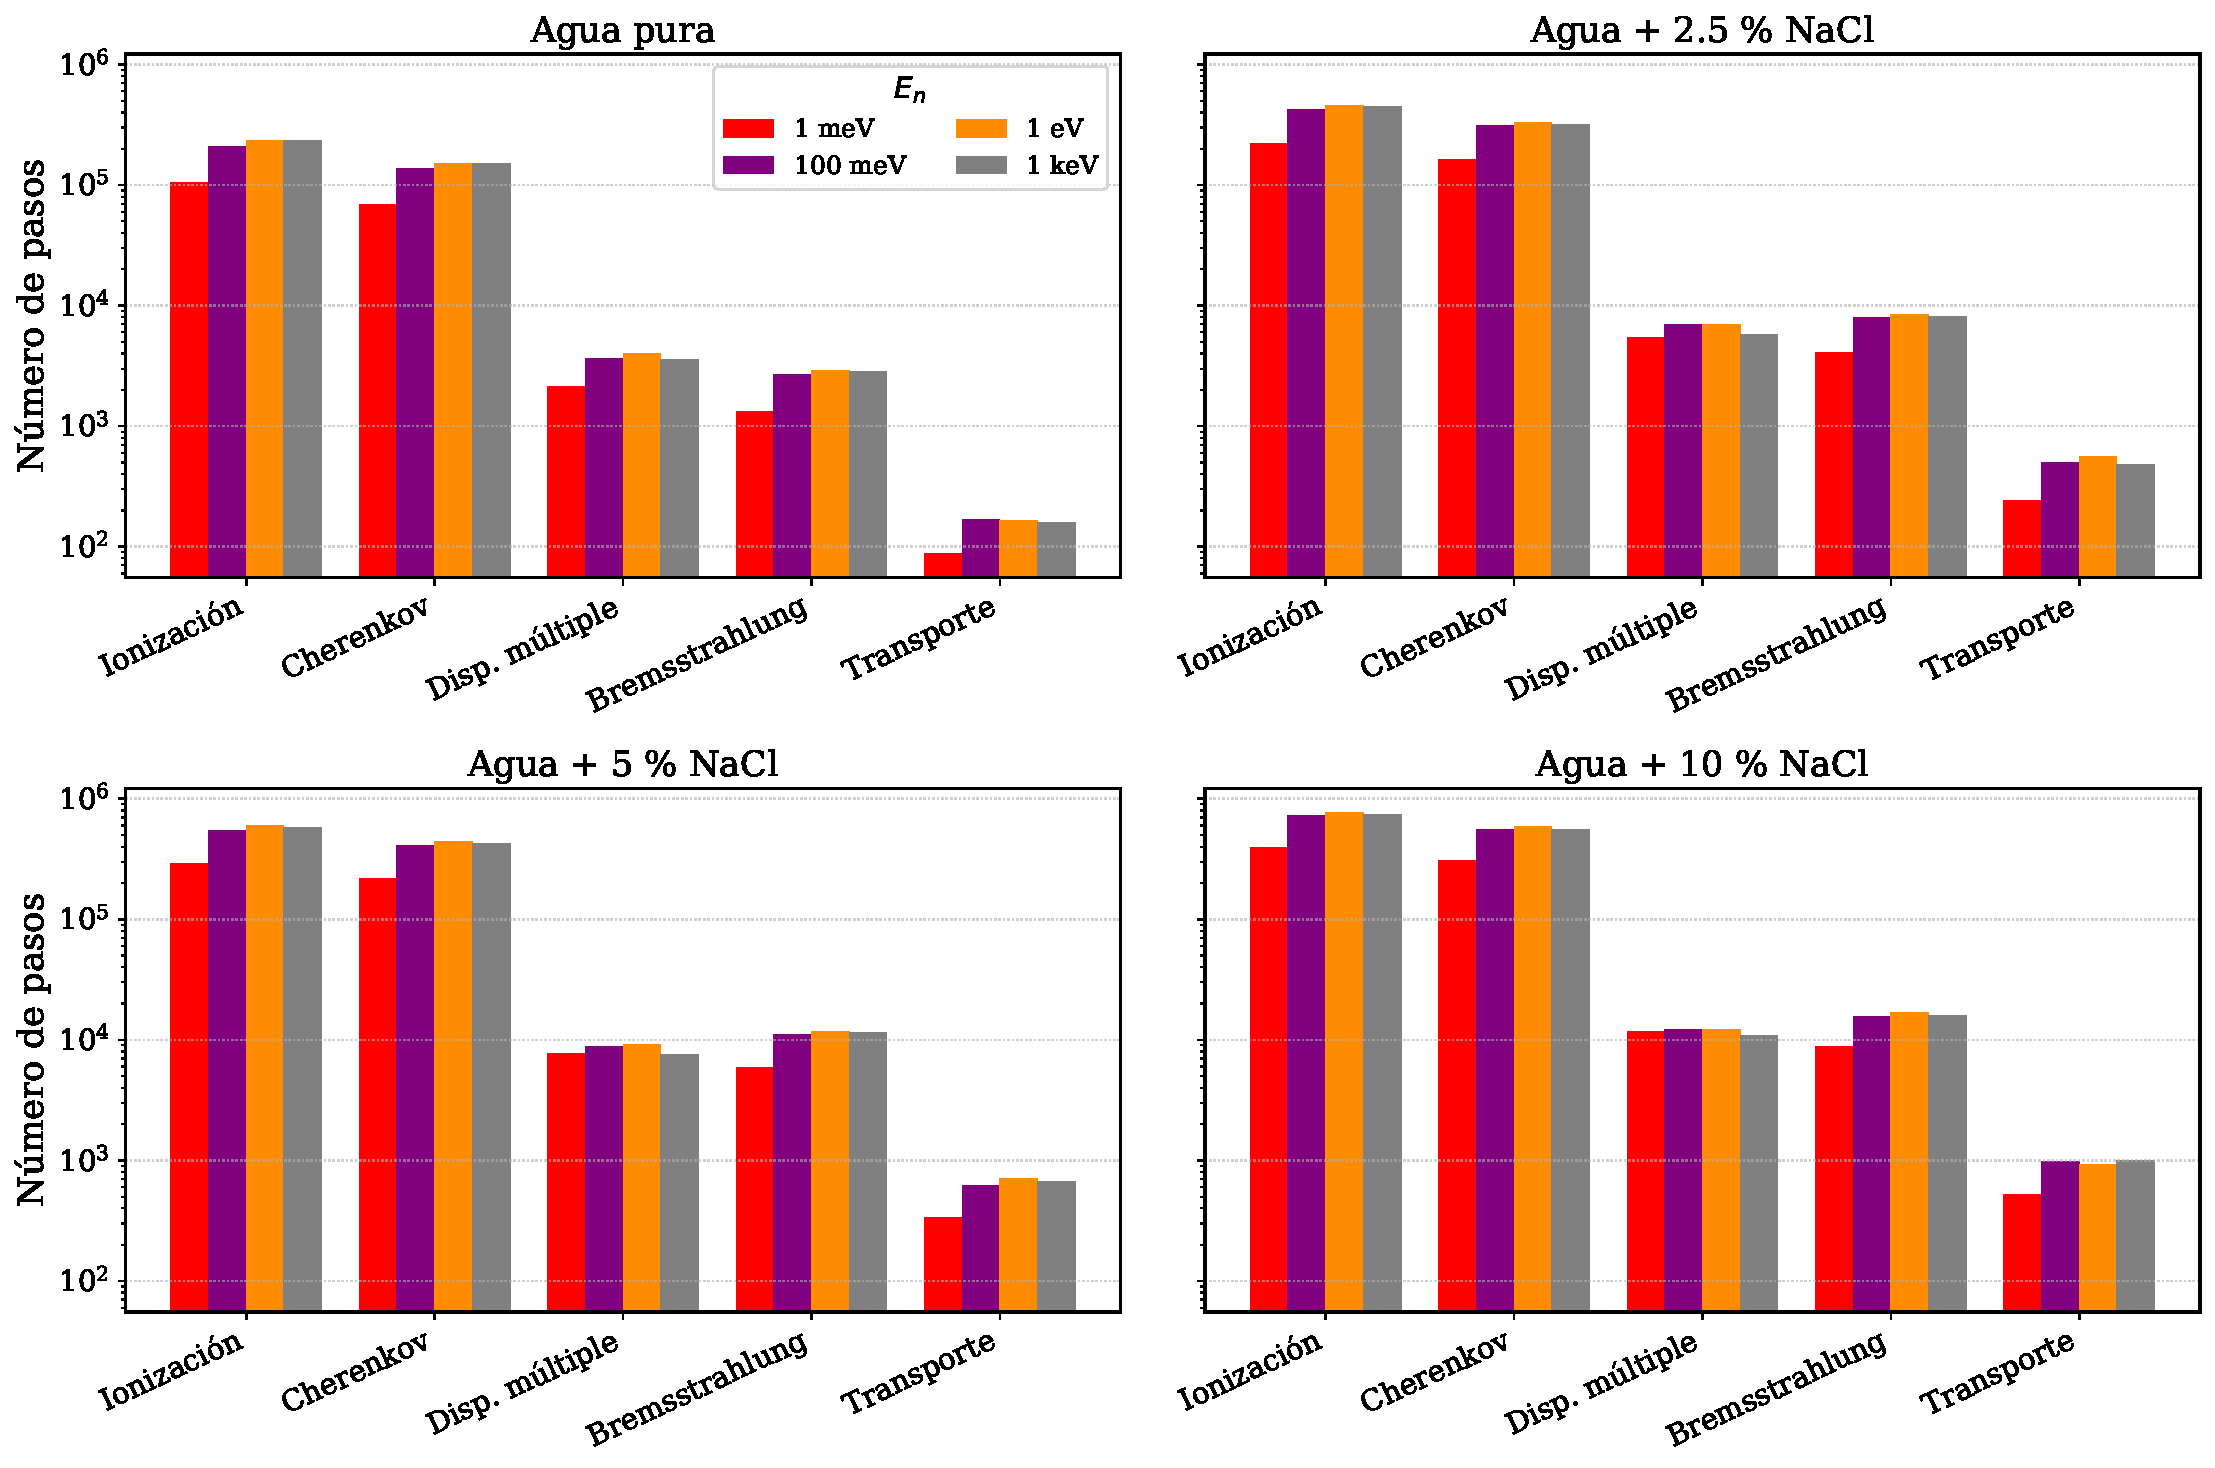
\includegraphics[width=0.95\linewidth]{fig_4_45_procesos_tanque.pdf}
\caption{Pasos por proceso de los $e^\pm$ en el tanque estricto para cuatro energías del neutrón (Fig.~4.45 de la tesis, regenerada). Se omiten \var{Scintillation} y la aniquilación (0--10 pasos por corrida).}
\label{fig:procesos}
\end{figure}

Los pasos de ionización y Cherenkov dominan (Tabla~\ref{tab:procesos}); la dispersión múltiple y el bremsstrahlung limitan del 1 al 3~\% de los pasos. Como el 87--88~\% de los pasos \var{eIoni} del tanque tienen $E=0$, la mayor parte de ellos es el último paso de electrones de baja energía que se detienen en uno o dos pasos (la energía media tras el primer paso es de 0.12~MeV en agua pura).

Los conteos absolutos crecen con la energía del neutrón y con la salinidad, pero por captura son casi constantes en $E_n$ (Fig.~\ref{fig:por-captura}): el aumento con $E_n$ entre 1~meV y 1~eV es el aumento del número de capturas en el tanque, que el informe de neutrones atribuye al albedo de los neutrones fríos. La dependencia con la salinidad es la de la fuente: con 10~\% de NaCl cada captura produce 2.2--2.4 veces más electrones y 2.7--2.8 veces más pasos \var{Cerenkov} que en agua pura.

\begin{figure}[H]
\centering
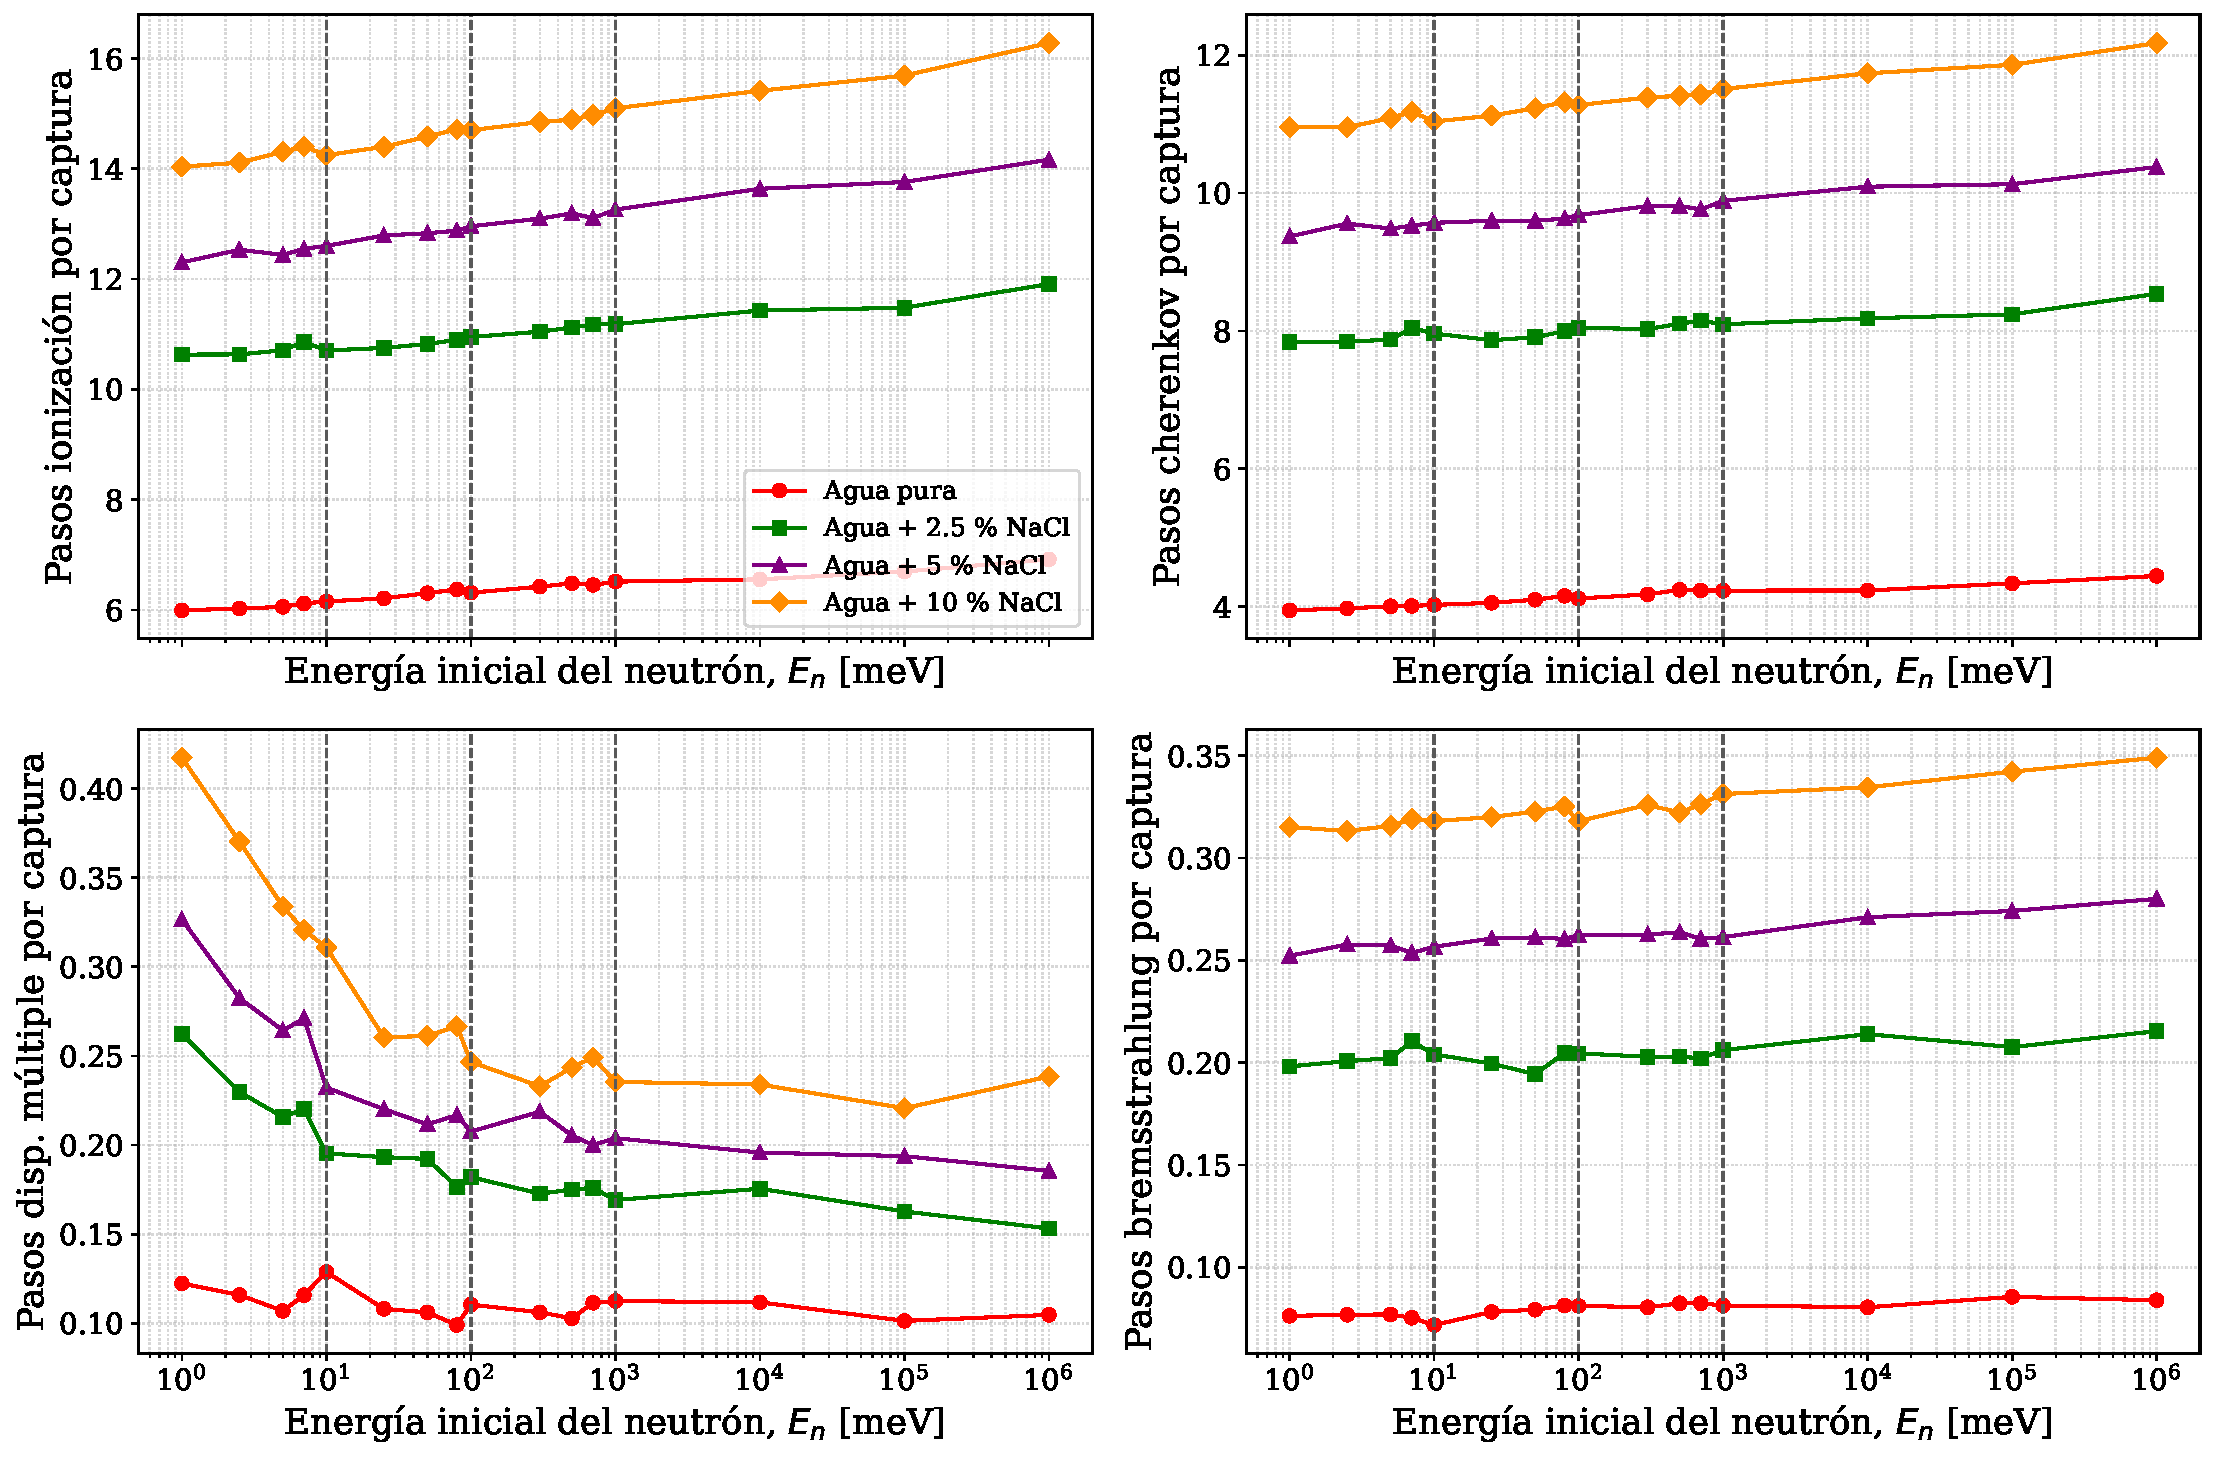
\includegraphics[width=0.95\linewidth]{fig_nueva_procesos_por_captura.pdf}
\caption{Pasos por captura en el tanque estricto frente a la energía del neutrón.}
\label{fig:por-captura}
\end{figure}

% =====================================================================
\section{El ``espectro de ionización'' (Fig.~4.46)}
\label{sec:eioni}

La Fig.~4.46 de la tesis es el histograma de la energía tras los pasos \var{eIoni} con $E\neq0$ (100 intervalos en 0--1.6~MeV, tanque estricto), y la tesis lo interpreta como el espectro de los electrones que ionizan el medio, con un máximo en 472~keV en agua pura que se desplaza a 492~keV con 2.5~\% de NaCl. La réplica (Fig.~\ref{fig:eioni}) reproduce la figura, pero no esa interpretación.

\begin{figure}[H]
\centering
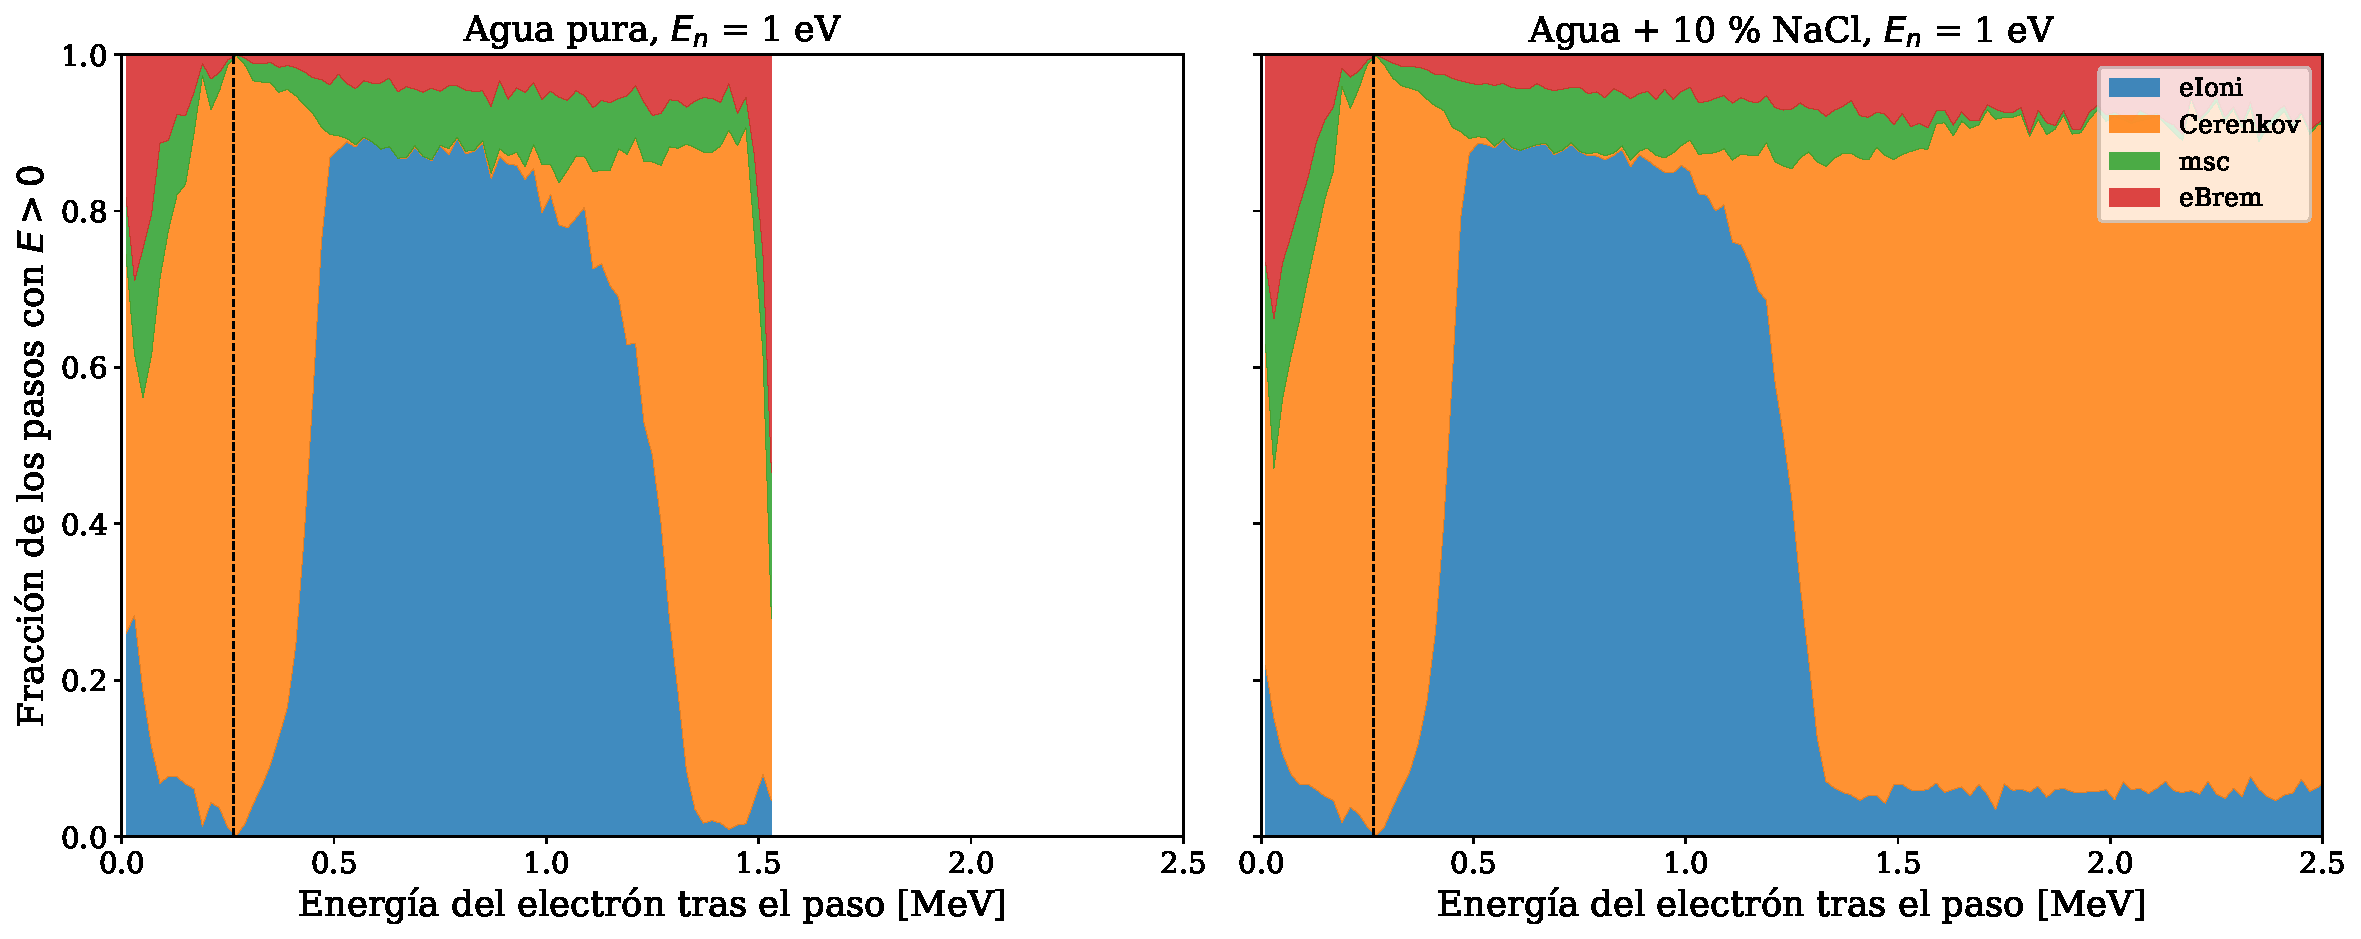
\includegraphics[width=0.95\linewidth]{fig_nueva_proceso_limitante.pdf}
\caption{Proceso que limita los pasos con $E>0$ en el tanque estricto según la energía del electrón tras el paso ($E_n$ = 1~eV). Línea discontinua: umbral Cherenkov del agua simulada (264.06~keV).}
\label{fig:limitante}
\end{figure}

Todos los electrones ionizan en todos sus pasos. Lo que cambia con la energía es qué proceso acorta el paso (Fig.~\ref{fig:limitante}): \var{G4Cerenkov} lo limita cerca del umbral, para que el electrón no lo cruce dentro del paso, y a energías altas, por el número máximo de fotones por paso; \var{eIoni} (producción de un electrón $\delta$ por encima del corte) solo gana entre unos 0.4 y 1.3~MeV. La curva de la Fig.~4.46 es la ventana en la que \var{eIoni} limita el paso: el flanco de 0.3--0.45~MeV y la caída en 1.3~MeV los fija el algoritmo de \textsc{Geant4}, no la física del depósito de energía, y la abscisa no es la energía depositada.

\begin{figure}[H]
\centering
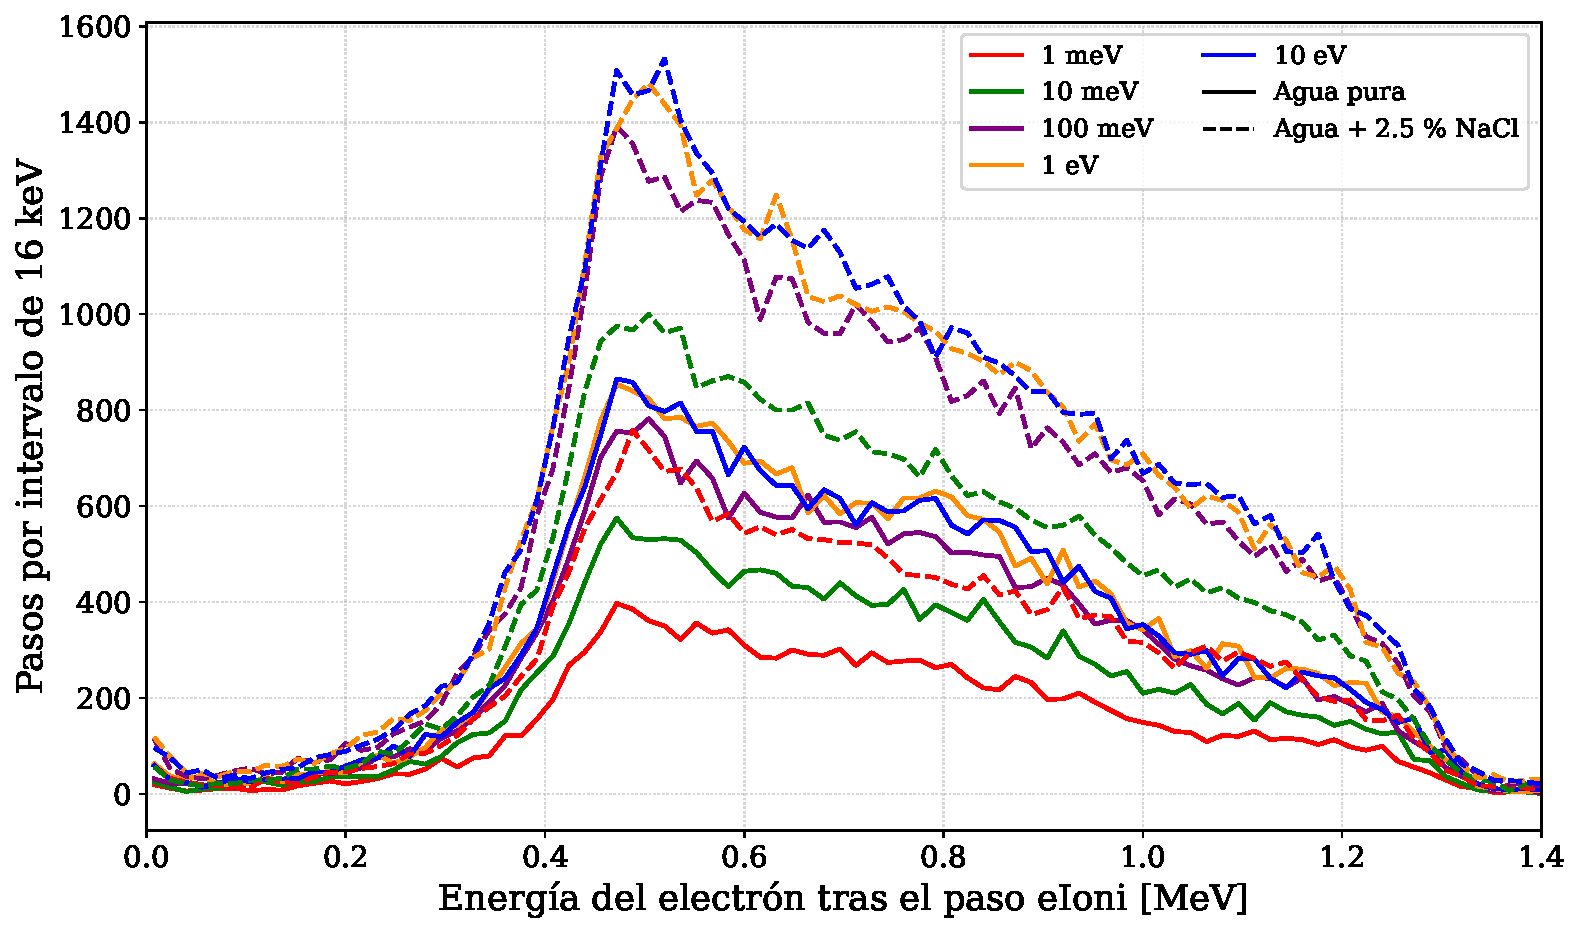
\includegraphics[width=0.85\linewidth]{fig_4_46_pasos_eIoni.pdf}
\caption{Energía tras los pasos \var{eIoni} con $E\neq0$ en el tanque estricto, agua pura y 2.5~\% de NaCl (réplica de la Fig.~4.46, mismas energías y la misma binning).}
\label{fig:eioni}
\end{figure}

Con intervalos de 16~keV el máximo salta entre 0.472, 0.488, 0.504 y 0.520~MeV de una energía del neutrón a otra en los dos medios; con un suavizado de 50~keV queda en 0.48--0.50~MeV en los cuatro medios, sin desplazamiento con la salinidad. Lo que sí cambia con el NaCl es la media, de 0.71~MeV en agua pura a 0.83--0.84, 0.85--0.86 y 0.86--0.88~MeV con 2.5, 5 y 10~\% de NaCl, por los electrones Compton más energéticos de los fotones del cloro.

% =====================================================================
\section{Energía inicial de los electrones y positrones}
\label{sec:inicial}

\begin{figure}[H]
\centering
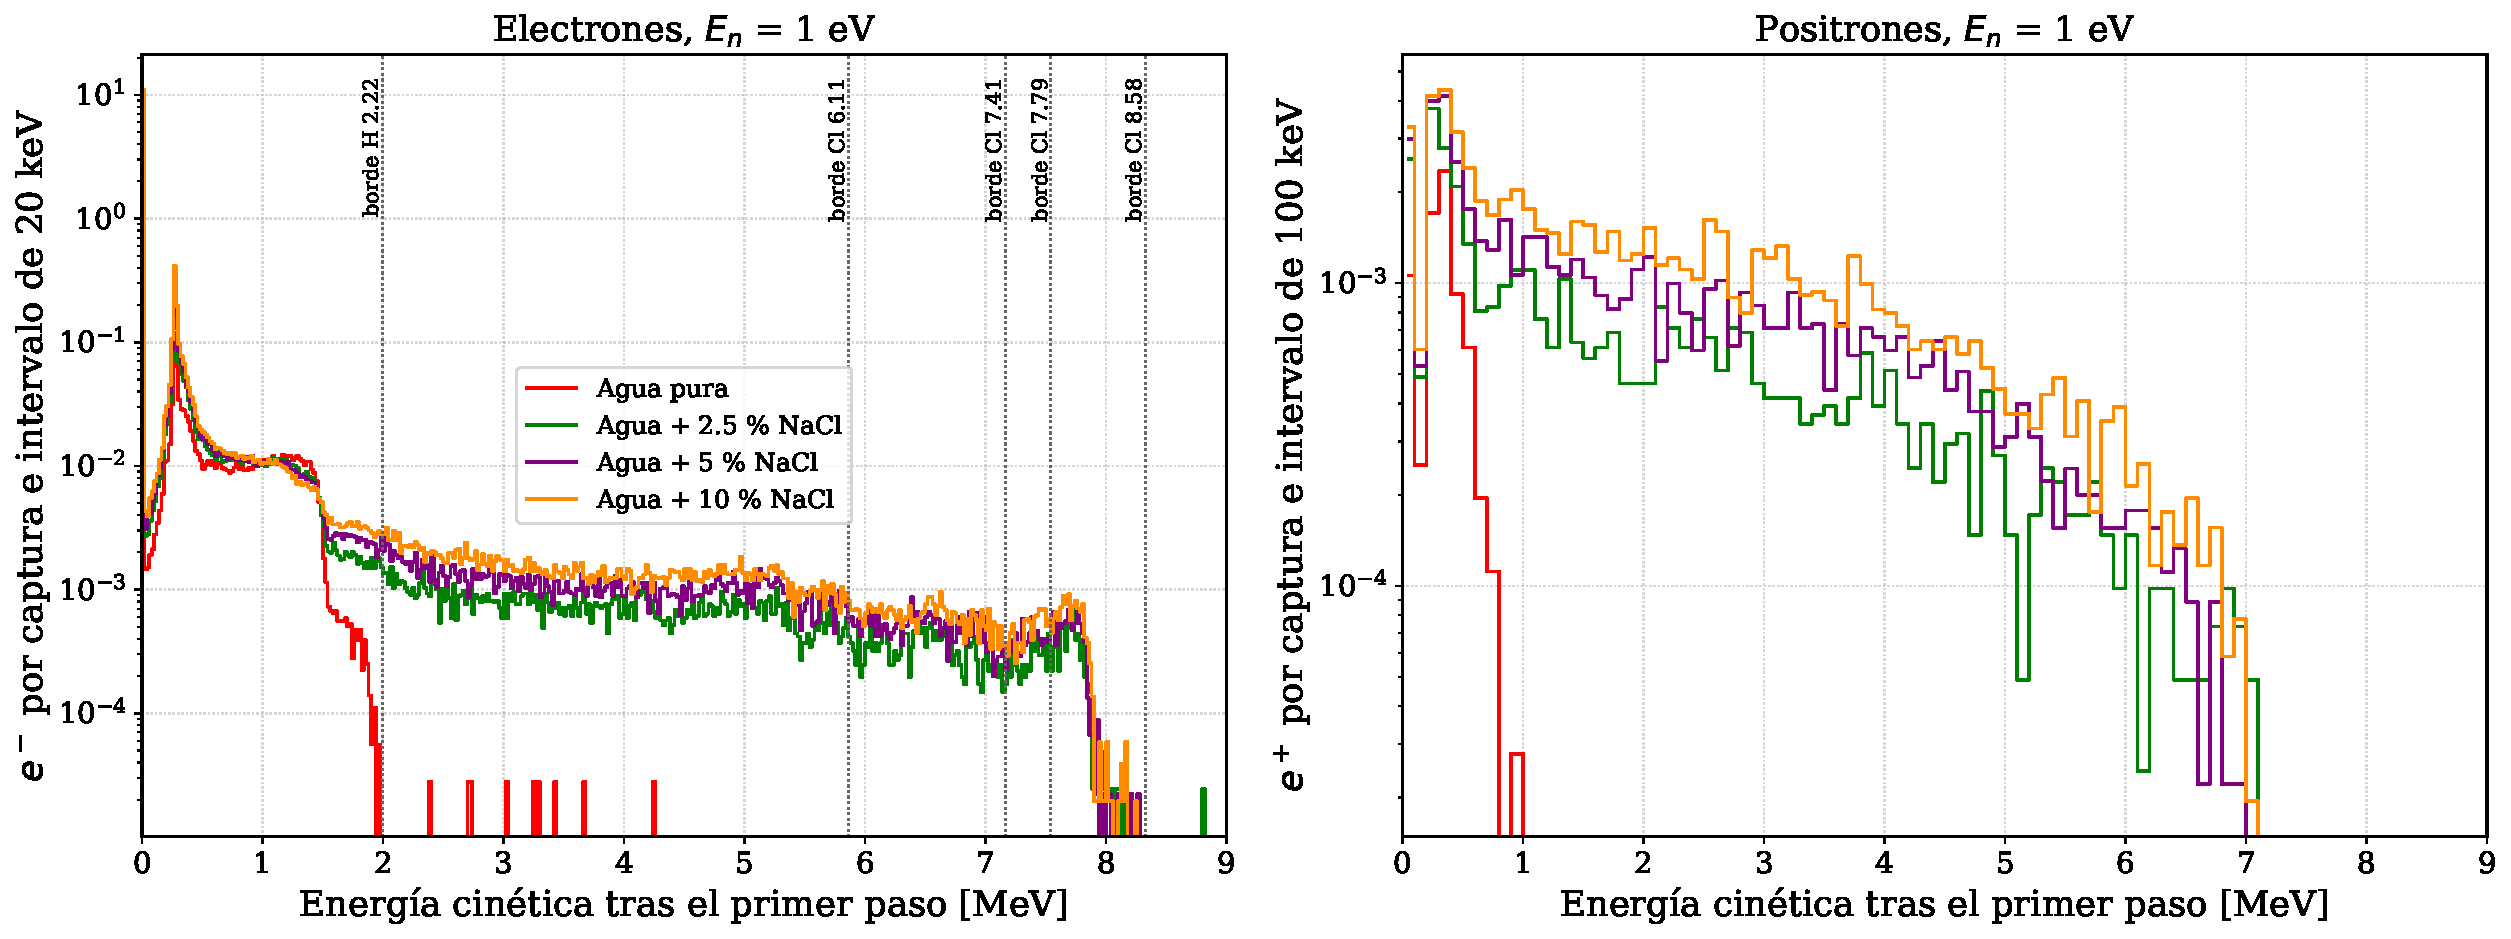
\includegraphics[width=\linewidth]{fig_nueva_energia_inicial.pdf}
\caption{Energía tras el primer paso de los $e^-$ y $e^+$ que nacen en el tanque, por captura ($E_n$ = 1~eV). Líneas punteadas: bordes Compton $T_\mathrm{max}=2E_\gamma^2/(m_ec^2+2E_\gamma)$ de las líneas de captura más intensas.}
\label{fig:inicial}
\end{figure}

La Fig.~\ref{fig:inicial} muestra la energía tras el primer paso, que es una cota inferior de la energía de producción. Tres rasgos lo confirman: el máximo en 264~keV (primeros pasos que \var{G4Cerenkov} detiene en el umbral), el gran número de trazas con $E=0$ (electrones de baja energía que se detienen en el primer paso) y la posición de los cortes, unos 0.4--0.5~MeV por debajo de los bordes Compton (1.99~MeV para la línea de 2.22~MeV del H; 8.33~MeV para la de 8.58~MeV del Cl). En agua pura casi ningún electrón supera los 2~MeV; con NaCl el espectro se extiende hasta 8~MeV con una meseta de los electrones Compton de las líneas de 6--8.6~MeV del cloro.

Los positrones proceden de la producción de pares. En agua pura son muy escasos (0.006--0.010 por captura, de la línea de 2.22~MeV, con energía cinética máxima de 1.2~MeV); con NaCl hay 0.04--0.08 por captura y su espectro llega a unos 7~MeV.

El espectro de producción de los electrones Compton se obtiene mejor de los fotones (energía perdida en cada paso \var{compt}), que se estudian en el informe de los fotones gamma; el archivo de electrones no permite reconstruirlo.

% =====================================================================
\section{El umbral Cherenkov en la simulación}
\label{sec:umbral}

Un electrón emite radiación Cherenkov si $\beta>1/n$, es decir, si su energía cinética supera
\[
E_\mathrm{U}=m_ec^2\left(\frac{1}{\sqrt{1-1/n^2}}-1\right).
\]
La Tabla~4.17 de la tesis da los índices de la literatura para las cuatro soluciones (1.3330, 1.3397, 1.3436 y 1.3594) y sus umbrales (261.81, 256.89, 254.11 y 243.36~keV); los cuatro umbrales se reproducen exactamente con esa fórmula. Pero la simulación de la Campaña~1 no usó esos índices. En \archivo{SaltyWCD.cc} el agua de los cuatro medios recibe la tabla óptica \var{waterPT1} de \archivo{Materials.cc}, con $n=1.33$ constante entre 2.08 y 4.20~eV, y el vidrio Pyrex del PMT tiene $n=1.47$. Los umbrales de la simulación son, por tanto,
\begin{align*}
E_\mathrm{U}(n=1.33)&=264.06~\mathrm{keV}\quad\text{en el agua de los cuatro medios},\\
E_\mathrm{U}(n=1.47)&=186.17~\mathrm{keV}\quad\text{en el Pyrex del PMT.}
\end{align*}

\begin{figure}[H]
\centering
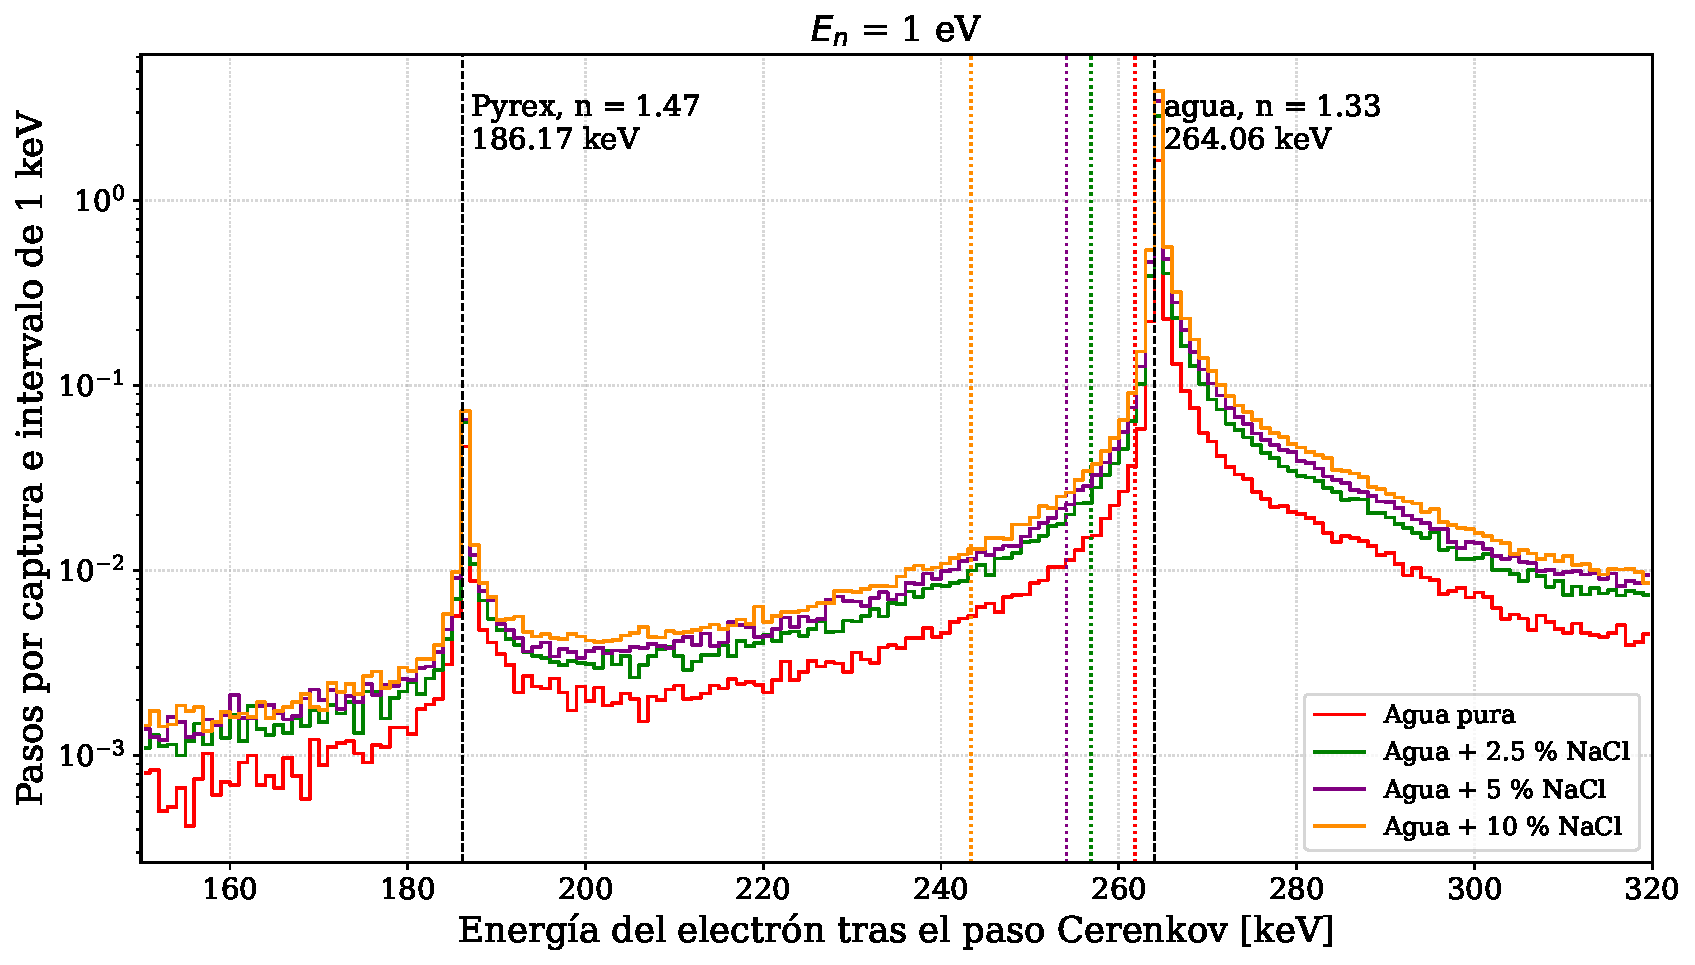
\includegraphics[width=0.9\linewidth]{fig_nueva_umbral_cherenkov.pdf}
\caption{Energía tras los pasos \var{Cerenkov} en el tanque estricto, por captura ($E_n$ = 1~eV). Discontinuas: umbrales de la simulación (agua, $n=1.33$; Pyrex, $n=1.47$). Punteadas: umbrales de la Tabla~4.17, que la simulación no usó.}
\label{fig:umbral}
\end{figure}

\var{G4Cerenkov} acorta el paso para que el electrón termine justo sobre el umbral del material en que se mueve; por eso la energía tras los pasos \var{Cerenkov} se acumula en los umbrales (Fig.~\ref{fig:umbral}). El máximo principal está en 264.06~keV en los cuatro medios y un segundo máximo, mucho más bajo, en 186.2~keV. El 13--16~\% de los pasos \var{Cerenkov} terminan bajo el umbral del agua: son los del Pyrex y pasos en los que la pérdida de energía fluctúa por encima de lo previsto por las tablas de alcance.

\subsection{Los pasos Cherenkov del Pyrex}
\label{sec:pyrex}

Los pasos \var{Cerenkov} con energía entre 180 y 190~keV (el 1.0--1.9~\% del total) se concentran a $z\approx1180$~mm y $r\approx90$~mm de media (Fig.~\ref{fig:pyrex}), en el domo del PMT; los demás pasos \var{Cerenkov} se reparten por la parte superior del tanque, donde ocurren las capturas. El segundo máximo del espectro es, por tanto, la emisión de los electrones que atraviesan el vidrio del fotomultiplicador, no un efecto del agua.

\begin{figure}[H]
\centering
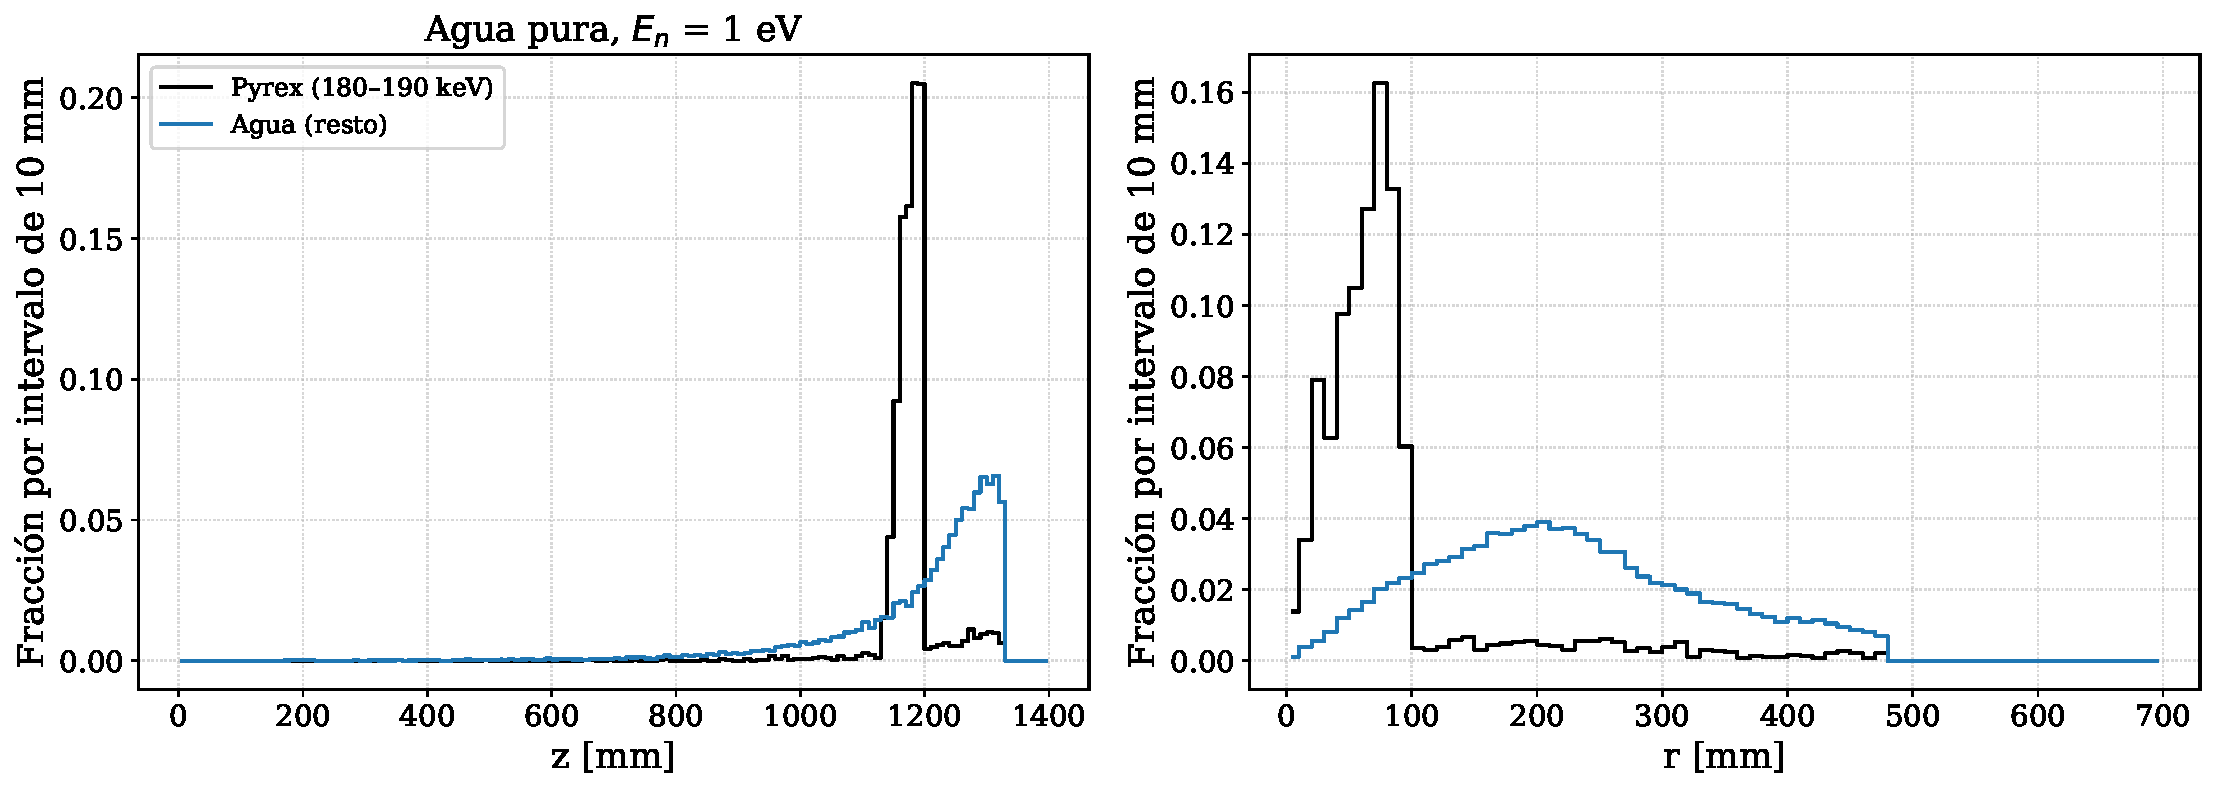
\includegraphics[width=0.9\linewidth]{fig_nueva_posicion_pyrex.pdf}
\caption{Distribución en $z$ y $r$ de los pasos \var{Cerenkov} con 180--190~keV (Pyrex) y del resto (agua); agua pura, $E_n$ = 1~eV.}
\label{fig:pyrex}
\end{figure}

% =====================================================================
\section{Ajuste fino del máximo (Fig.~4.47, Tabla~4.18)}
\label{sec:ajuste}

La tesis ajusta el máximo con una gaussiana más un fondo lineal en $\pm4.5$~keV alrededor del intervalo más poblado de un histograma de 0.04~keV, y obtiene 264.10~keV en agua pura y 264.11~keV con NaCl. El mismo procedimiento sobre los datos sin desplazar da 264.085--264.088~keV en las cinco energías y los cuatro medios (Tabla~\ref{tab:ajuste}), a menos de un intervalo del valor de la tesis. La pequeña diferencia con el umbral analítico (0.03~keV) se debe a que el ajuste simétrico se aplica a un borde: la distribución empieza abruptamente en 264.06~keV y decae hacia energías mayores (Fig.~\ref{fig:ajuste}).

\begin{figure}[H]
\centering
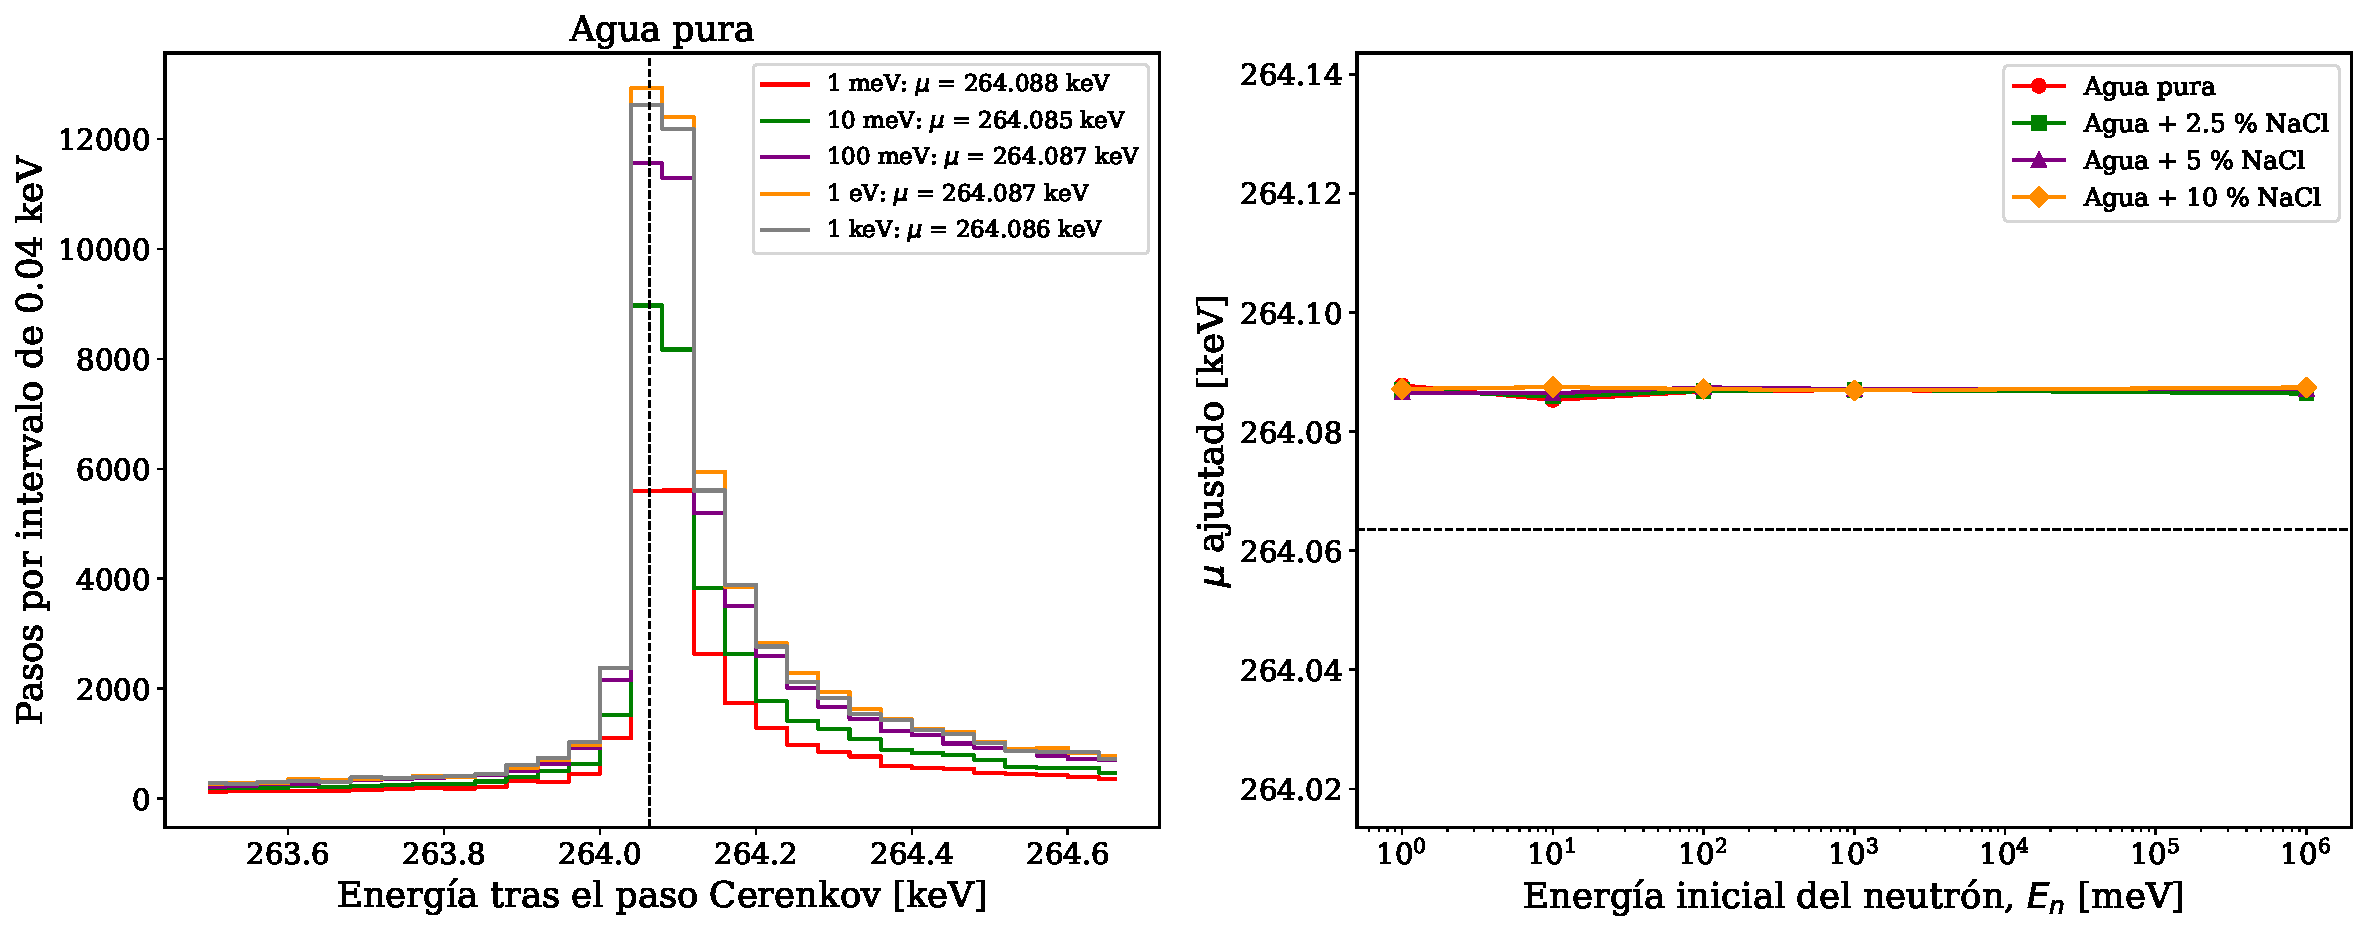
\includegraphics[width=\linewidth]{fig_4_47_ajuste_fino_cherenkov.pdf}
\caption{Izquierda: máximo del espectro de los pasos \var{Cerenkov} en agua pura (intervalos de 0.04~keV; línea discontinua: umbral para $n=1.33$). Derecha: centro ajustado para las cinco energías y los cuatro medios.}
\label{fig:ajuste}
\end{figure}

\begin{table}[H]
\centering\small
\caption{Centro $\mu$ [keV] del ajuste del máximo Cherenkov (incertidumbre estadística 0.0013--0.0014~keV; $\sigma$ = 0.041--0.044~keV).}
\label{tab:ajuste}
\begin{tabular}{@{}lrrrr@{}}
\toprule
$E_n$ & Agua pura & 2.5~\% NaCl & 5~\% NaCl & 10~\% NaCl \\
\midrule
\csname @@input\endcsname \tablas/tabla_ajuste_cherenkov.tex
\bottomrule
\end{tabular}
\end{table}

Dos consecuencias para la tesis:
\begin{itemize}
  \item La coincidencia del 0.87~\% entre el máximo (264.1~keV) y el umbral de la Tabla~4.17 para el agua pura (261.81~keV) no es una validación: refleja solo la diferencia entre $n=1.333$ (literatura) y $n=1.33$ (simulación). Con el índice de la simulación, la coincidencia es exacta.
  \item Las diferencias de 2.81, 3.94 y 8.53~\% con los umbrales de las soluciones de NaCl no son un efecto del medio: la simulación usó el mismo índice en todos. La tesis ya reconoce que la dependencia del umbral con la concentración no quedó incorporada; aquí se identifica la causa (la tabla \var{waterPT1}) y el valor del índice usado.
\end{itemize}

\textbf{Datos desplazados en el análisis original.} El notebook \archivo{Ajuste-cherenkov-AP-1me-1keV.ipynb} restó a todas las energías \var{Cerenkov} de los medios con NaCl una constante (5.6128, 9.3931 y 15.3931~keV para 2.5, 5 y 10~\%) y escribió los resultados en archivos nuevos (\archivo{Cerenkov-A25NaCl-*.txt}, etc.), con lo que los máximos de esos medios aparecían en 258.5, 254.7 y 248.7~keV. Ese desplazamiento no tiene base física y debe descartarse. La tesis da los máximos sin desplazar (Tabla~4.18) y, desde la revisión del 6 de octubre de 2026, la nota de la Tabla~4.19 da la ventana sin desplazar (Sección~\ref{sec:ventana}). Las figuras \archivo{Ajuste-fino-pico-Cherenkov-cinco-energias-A25NaCl.pdf} y \archivo{Ajuste-fino-pico-Cherenkov-cuatro-medios.pdf} de la carpeta de figuras de la tesis no se usan en el texto actual y deben conservarse fuera de él.

% =====================================================================
\section{Pasos en la ventana del máximo (Tabla~4.19)}
\label{sec:ventana}

La Tabla~4.19 de la tesis cuenta los pasos \var{Cerenkov} del tanque estricto con energía en la ventana del ajuste. En agua pura la ventana es 0.2596--0.2686~MeV sobre los datos crudos. En los medios con NaCl la nota de la tabla da ventanas desplazadas (0.25396--0.26296, 0.25020--0.25920 y 0.24420--0.25320~MeV) que se aplicaron a los datos desplazados; sobre los datos crudos equivalen a la misma ventana del agua pura con diferencias de 0.03~keV en los bordes. Con esa definición, las 20 cifras se reproducen exactamente (Tabla~\ref{tab:ventana}), igual que la fracción del 59.257--59.419~\% de los pasos \var{Cerenkov} de agua pura dentro de la ventana.

\begin{table}[H]
\centering\small
\setlength{\tabcolsep}{4pt}
\caption{Pasos \var{Cerenkov} en la ventana del máximo (Tabla~4.19 de la tesis, reproducida) y por captura.}
\label{tab:ventana}
\begin{tabular}{@{}lrrrrrrrr@{}}
\toprule
& \multicolumn{2}{c}{Agua pura} & \multicolumn{2}{c}{2.5~\% NaCl} & \multicolumn{2}{c}{5~\% NaCl} & \multicolumn{2}{c}{10~\% NaCl} \\
$E_n$ & $N$ & $N/N_\mathrm{Cap}$ & $N$ & $N/N_\mathrm{Cap}$ & $N$ & $N/N_\mathrm{Cap}$ & $N$ & $N/N_\mathrm{Cap}$ \\
\midrule
\csname @@input\endcsname \tablas/tabla_ventana.tex
\bottomrule
\end{tabular}
\end{table}

Tres precisiones sobre la lectura de la tesis:
\begin{itemize}
  \item $N$ cuenta pasos, no electrones: una traza emisora tiene de media 4.3--4.9 pasos \var{Cerenkov}, de los que unos 2.6 caen en la ventana.
  \item La dependencia no monótona con $E_n$ (máximo a 1~eV y descenso a 1~keV) es la del número de capturas en el tanque. Por captura, el conteo crece poco (de 2.34 a 2.64 en agua pura); la explicación de la tesis, una mayor probabilidad de interacción del neutrón con la energía, no corresponde a estos datos.
  \item La constancia de la fracción dentro de la ventana es automática: la ventana contiene el borde del umbral, cuya forma fija el algoritmo de limitación del paso.
\end{itemize}

% =====================================================================
\section{Rendimientos por captura}
\label{sec:rendimientos}

\begin{table}[H]
\centering\small
\caption{Rendimientos por captura en el tanque (intervalo sobre las 16 energías del neutrón).}
\label{tab:rendimientos}
\begin{tabular}{@{}lrrrr@{}}
\toprule
Por captura & Agua pura & 2.5~\% NaCl & 5~\% NaCl & 10~\% NaCl \\
\midrule
\csname @@input\endcsname \tablas/tabla_rendimientos.tex
\bottomrule
\end{tabular}
\end{table}

\begin{figure}[H]
\centering
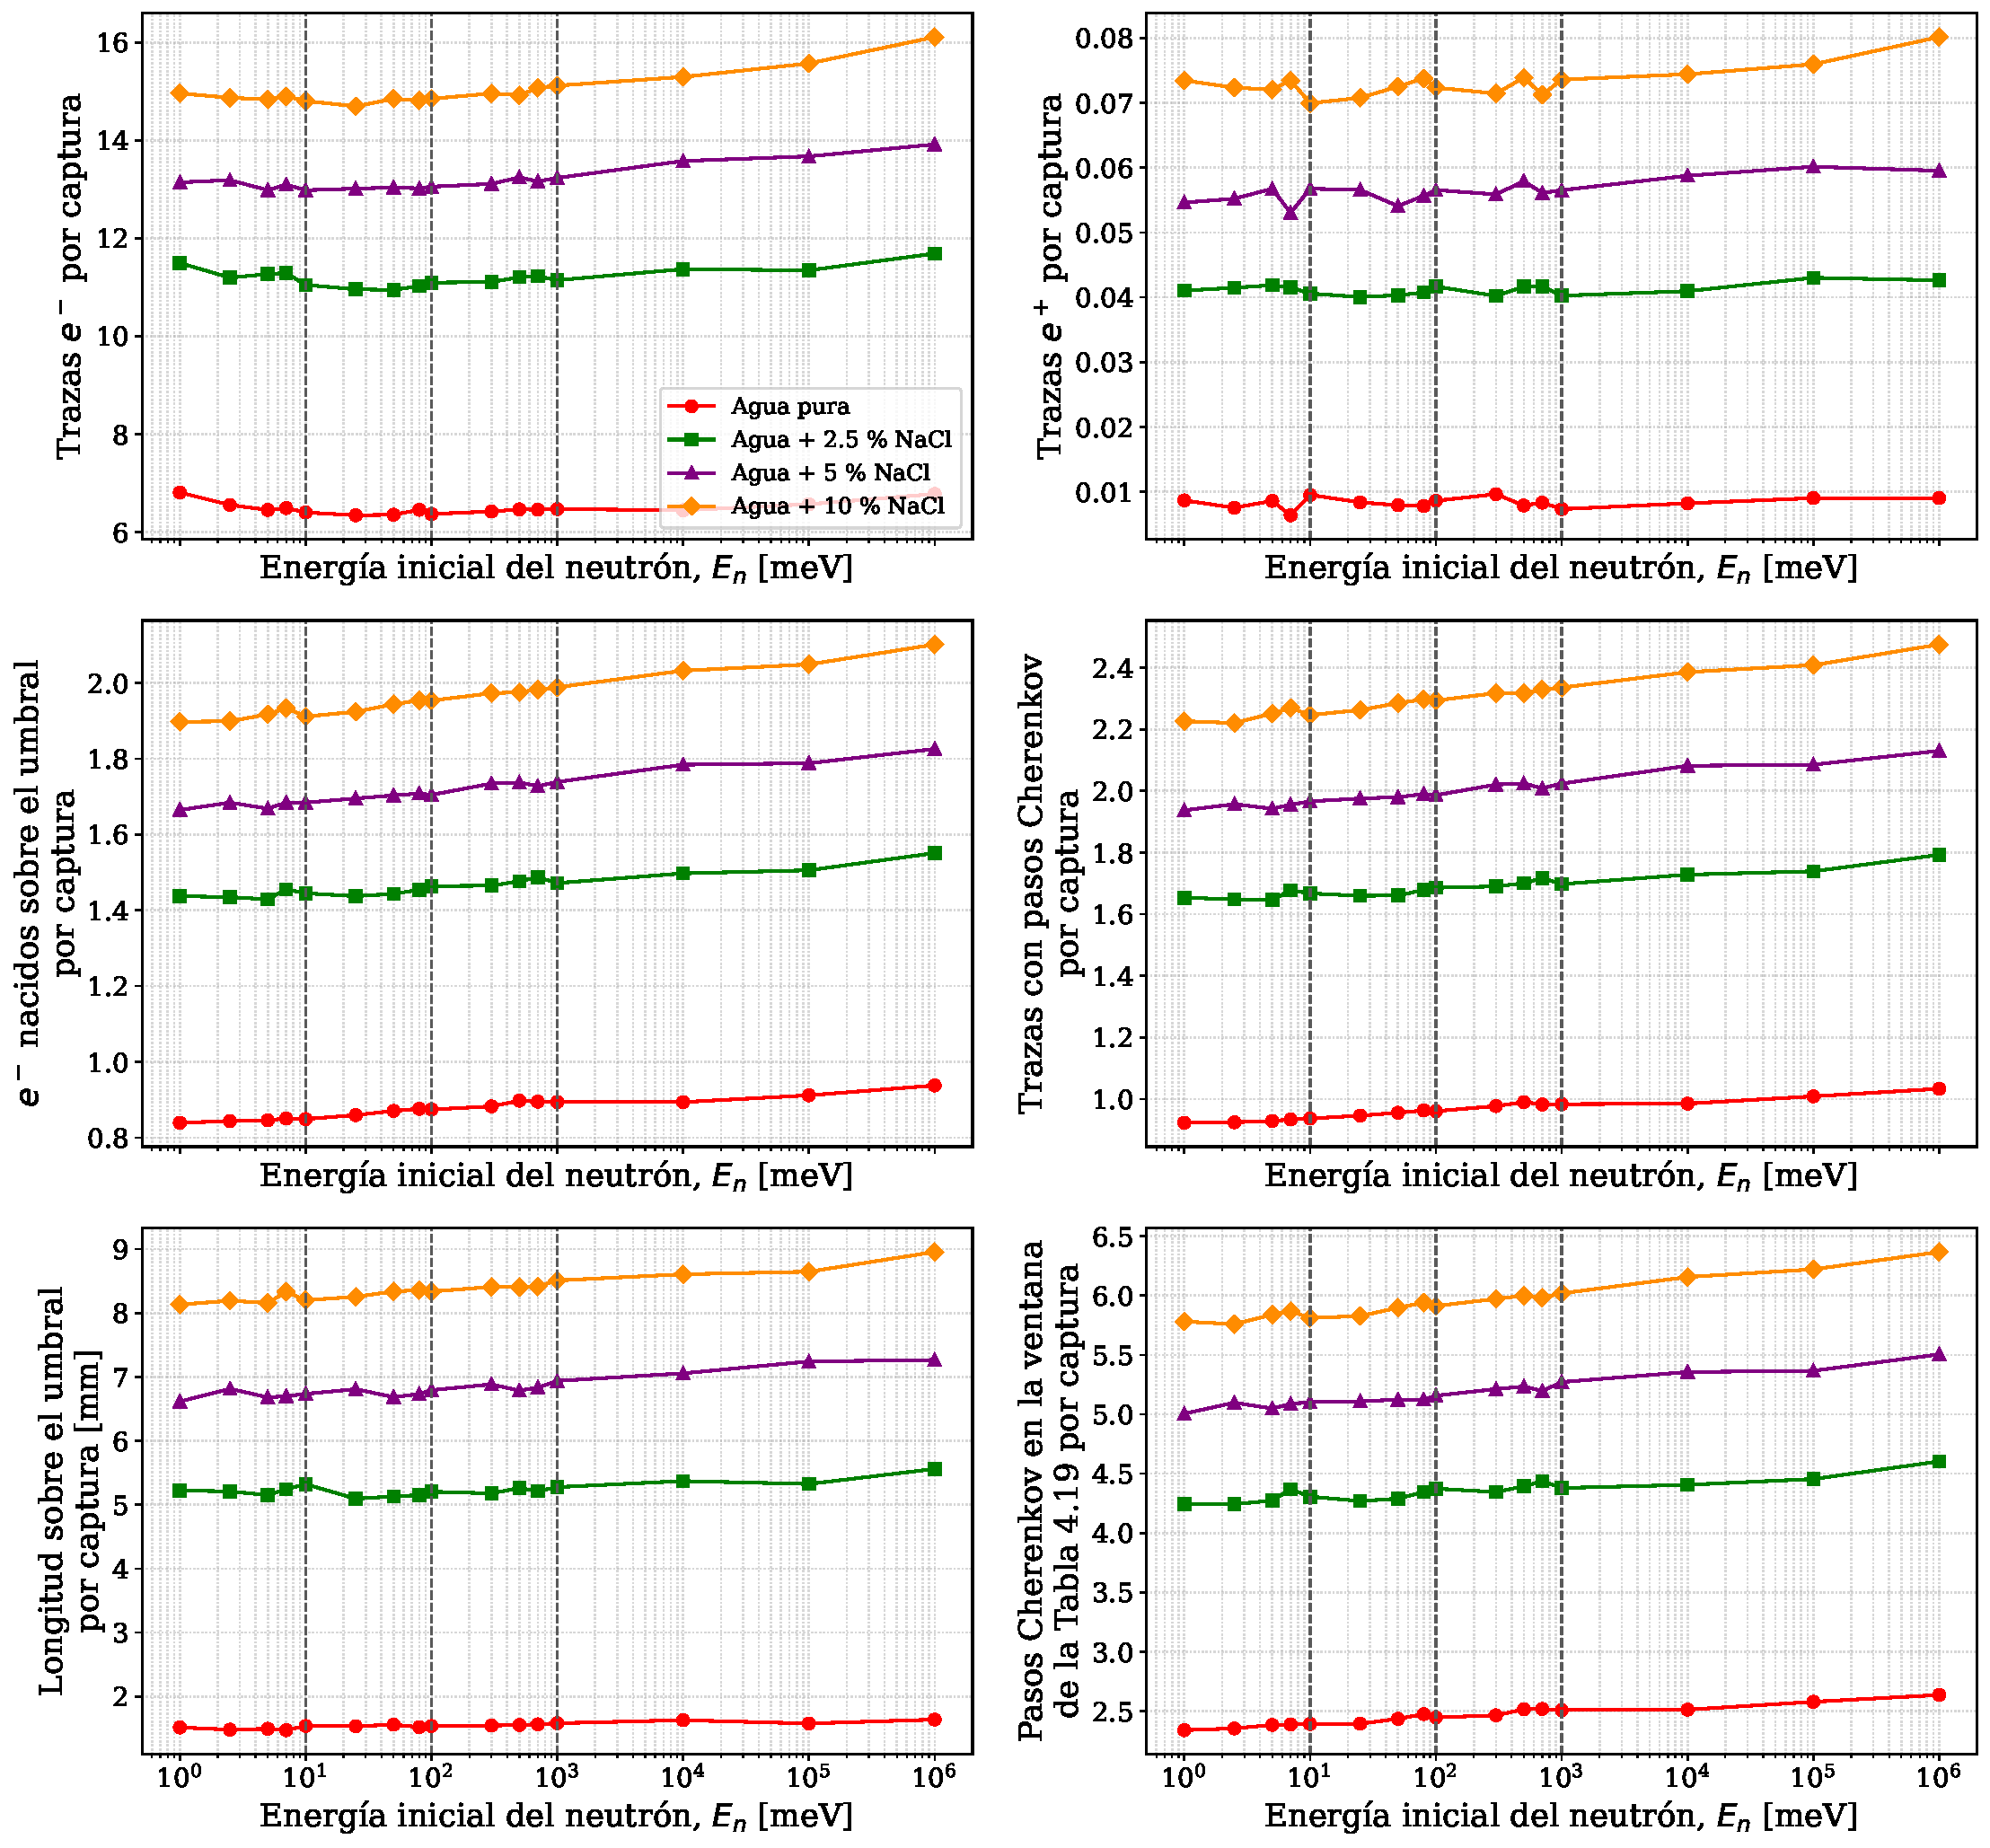
\includegraphics[width=0.95\linewidth]{fig_nueva_rendimientos_por_captura.pdf}
\caption{Rendimientos por captura frente a la energía del neutrón.}
\label{fig:rendimientos}
\end{figure}

Los rendimientos por captura (Tabla~\ref{tab:rendimientos}, Fig.~\ref{fig:rendimientos}) dependen sobre todo del medio y apenas de la energía del neutrón: entre 1~meV y 1~keV el número de electrones cambia menos del 8~\% y las magnitudes ligadas al umbral crecen un 10--12~\%. Con respecto al agua pura, el 10~\% de NaCl multiplica por captura el número de electrones por 2.2--2.4, el de trazas emisoras por 2.3--2.4 y la longitud de trayectoria sobre el umbral por 5.3--5.7. La longitud crece más que el número de emisores porque los electrones Compton de las líneas del cloro son más energéticos: una traza emisora recorre de media 1.6~mm sobre el umbral en agua pura y 3.6~mm con 10~\% de NaCl. La longitud no incluye el primer paso de cada traza, por lo que es una cota inferior y el cociente entre medios debe confirmarse antes de usarlo para predecir el número de fotones Cherenkov.

Hay que recordar dos limitaciones heredadas de las etapas anteriores: las cascadas de captura del $^{35}$Cl simuladas no conservan la energía (en el informe de los fotones gamma, la energía gamma por captura aumenta un 12--17~\% en los medios con NaCl), lo que sobrestima en una proporción parecida los electrones de alta energía de esos medios; y el índice de refracción es el mismo en todos los medios, de modo que las diferencias de luz entre medios en esta campaña proceden solo de la fuente y del transporte, no de la óptica de la solución.

% =====================================================================
\section{Energía de todos los pasos (Figs.~E.3 y E.4)}

\begin{figure}[H]
\centering
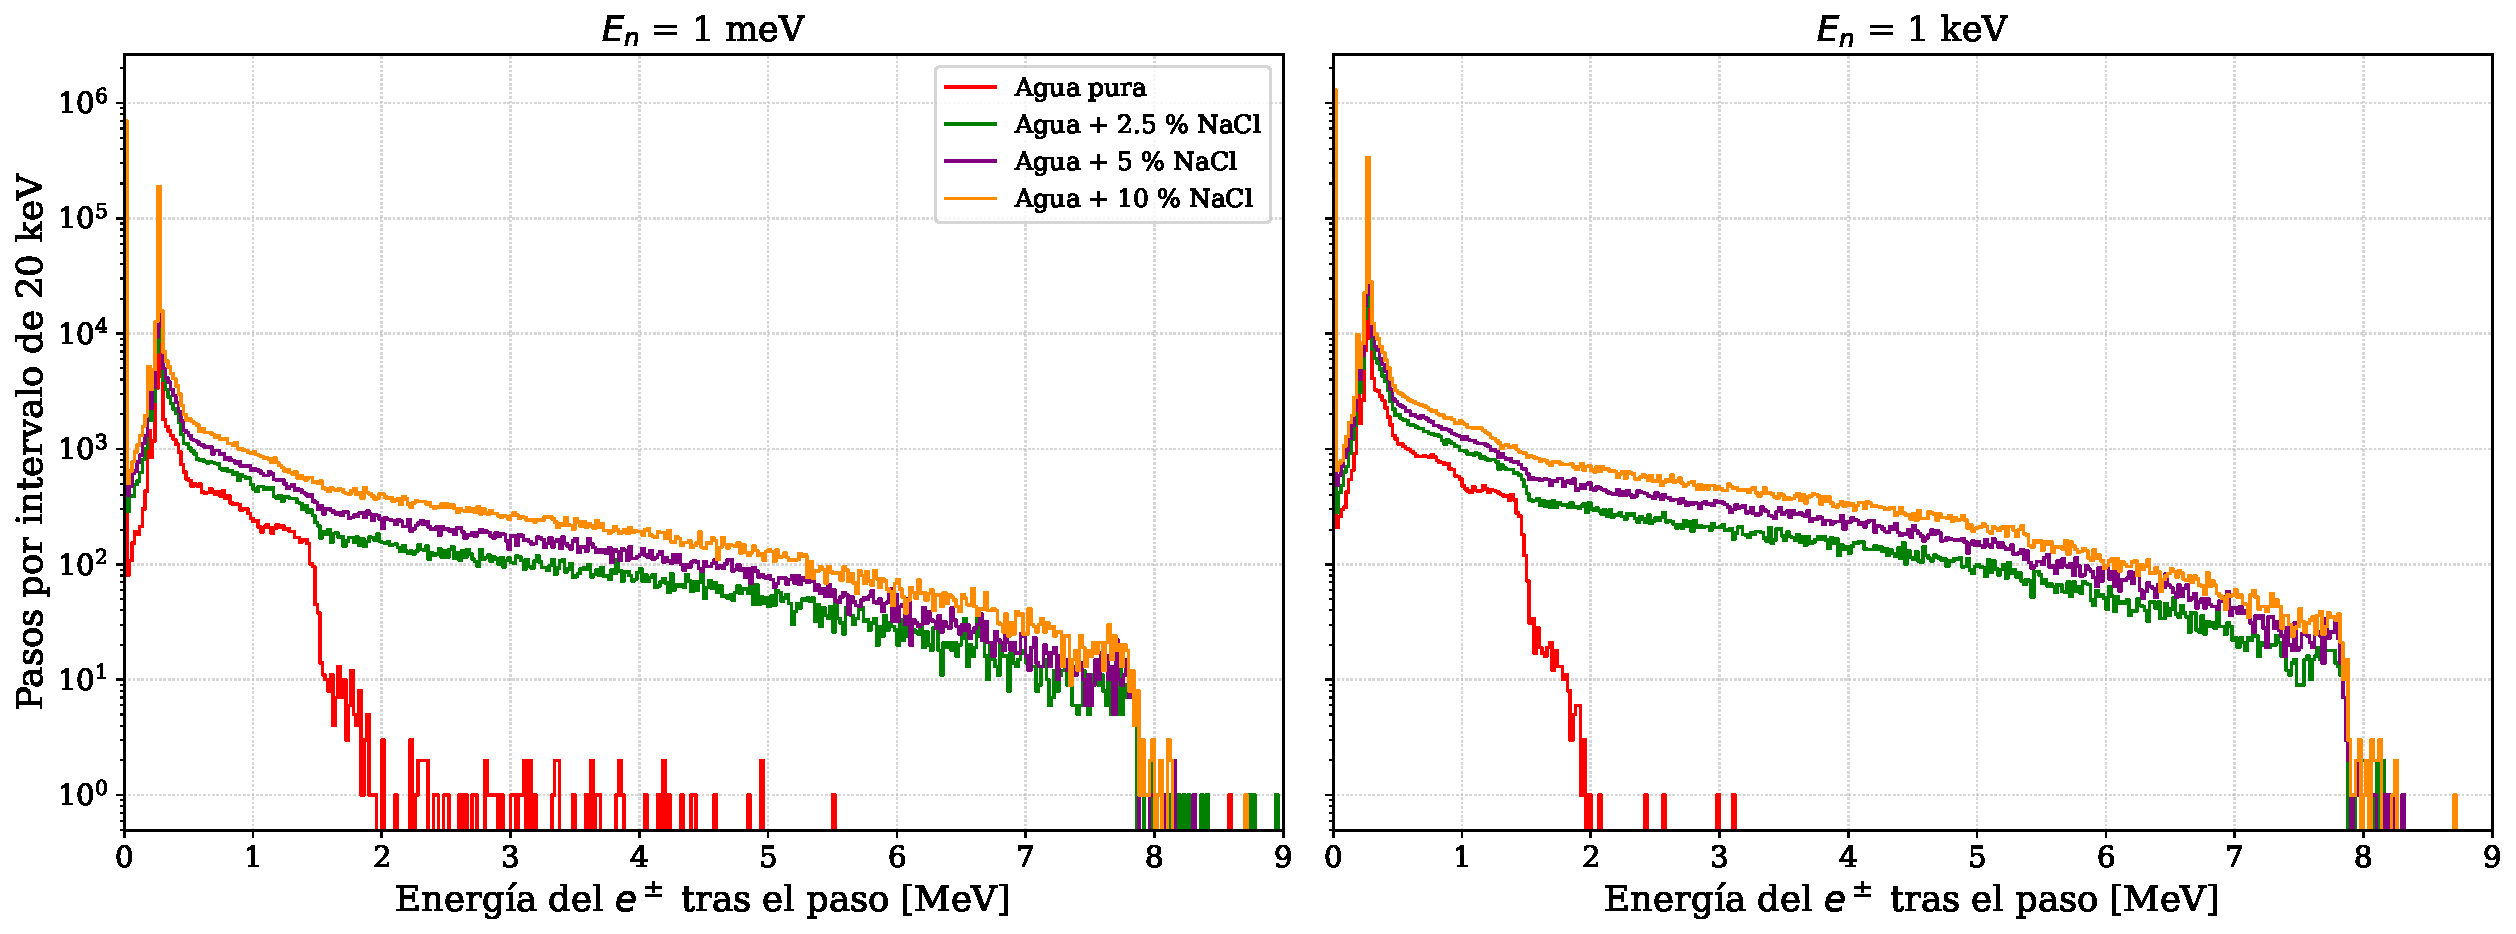
\includegraphics[width=\linewidth]{fig_E3_E4_pasos_tanque.pdf}
\caption{Energía tras cada paso de los $e^\pm$ en el tanque, a 1~meV y 1~keV (Figs.~E.3 y E.4 de la tesis, regeneradas).}
\label{fig:pasos}
\end{figure}

El espectro de todos los pasos (Fig.~\ref{fig:pasos}) está dominado por los pasos con $E=0$ y por el borde del umbral; el continuo por encima refleja la energía de los electrones a lo largo de sus trayectorias y, como en la Fig.~\ref{fig:inicial}, termina cerca de 2~MeV en agua pura y de 8~MeV con NaCl.

% =====================================================================
\section{Verificación frente a la tesis}
\label{sec:verificacion}

\subsection{Definiciones reconstruidas}

\begin{itemize}
  \item \textbf{Fig.~4.45 y Tabla~E.1:} filas del proceso en el tanque estricto.
  \item \textbf{Fig.~4.46:} filas \var{eIoni} con $E\neq0$ en el tanque estricto; 100 intervalos en 0--1.6~MeV.
  \item \textbf{Tabla~4.17:} fórmula del umbral con los índices de la literatura.
  \item \textbf{Fig.~4.47 y Tabla~4.18:} filas \var{Cerenkov} del tanque estricto; gaussiana más fondo lineal en $\pm4.5$~keV sobre intervalos de 0.04~keV.
  \item \textbf{Tabla~4.19:} filas \var{Cerenkov} del tanque estricto en la ventana de la Sección~\ref{sec:ventana}.
\end{itemize}

\subsection{Resultado}

\begin{table}[H]
\centering\small
\caption{Cifras de electrones de la tesis recalculadas desde los archivos crudos. Compatibles: a menos de un intervalo de 0.04~keV.}
\label{tab:verif}
\begin{tabular}{@{}lrrrr@{}}
\toprule
Magnitud & Cifras & Iguales & Compatibles & Distintas \\
\midrule
\csname @@input\endcsname \tablas/tabla_verificacion_resumen.tex
\bottomrule
\end{tabular}
\end{table}

\begin{table}[H]
\centering\small
\caption{Cifras que difieren.}
\label{tab:verif-dif}
\begin{tabular}{@{}lllrr@{}}
\toprule
Magnitud & $E_n$ & Medio & Tesis & Reproducido \\
\midrule
\csname @@input\endcsname \tablas/tabla_verificacion_diferencias.tex
\bottomrule
\end{tabular}
\end{table}

De 152 cifras, 118 coinciden exactamente y 20 dentro de un intervalo (Tabla~\ref{tab:verif}). Las ocho diferencias de la Tabla~E.1 son de transcripción: a 1~meV con 2.5 y 5~\% de NaCl las columnas \var{msc} y \var{eBrem} están intercambiadas; a 100~meV, \var{msc} en agua pura (2\,132), \var{eBrem} con 10~\% (8\,858) y \var{Transportation} con 2.5~\% (240) repiten los valores de 1~meV, y \var{eBrem} en agua pura (3\,668) es el valor de \var{msc}. La Tabla~\ref{tab:procesos} da los valores correctos, ya incorporados en la tesis. Los seis máximos de la Fig.~4.46 que difieren reflejan que la posición del máximo de un intervalo de 16~keV no es estable (Sección~\ref{sec:eioni}); la tesis da un único valor por medio.

% =====================================================================
\subsection{Correcciones incorporadas en la tesis}

El 6 de octubre de 2026 se incorporaron en la tesis: las ocho celdas de la Tabla~E.1 y su pie; la Fig.~4.45 regenerada desde los resúmenes, con el texto que explica que los conteos son pasos según el proceso que los limita y qué es \var{Scintillation}; la Fig.~4.46 regenerada con el eje correcto y la interpretación de la Sección~\ref{sec:eioni} (sin el desplazamiento de 472 a 492~keV); la explicación del máximo Cherenkov por el índice $n=1.33$ de la tabla \var{waterPT1} y del segundo máximo por el Pyrex; la nota de la Tabla~4.19 y la explicación de su dependencia con $E_n$ por el número de capturas; y, en la metodología, la aclaración de que la Campaña~1 usó el mismo índice en los cuatro medios.

\section{Reproducibilidad}

Desde la carpeta \archivo{analysis/campana-1_respuesta-electromagnetica_seccion-4.2/} del repositorio:
\begin{lstlisting}
python3 procesar_electrones.py <carpeta Electrones> resultados_electrones 12
python3 verificar_tesis_electrones.py <carpeta Electrones> resultados_electrones \
  resultados_electrones/verificacion_tesis_electrones.tsv
python3 construir_notebook_electrones.py
jupyter nbconvert --to notebook --execute figuras_electrones_seccion_4.2.ipynb
python3 tablas_informe_electrones.py resultados_electrones \
  ../campana-1_neutrones-monoenergeticos_seccion-4.2/resultados/resumen_campana.tsv \
  ../../docs/technical-reports/campana-1_sin-S-alpha-beta/tablas-electrones-secundarios
\end{lstlisting}
El procesamiento tarda 35~segundos con doce procesos y escribe 6~MB; la verificación, unos diez segundos (relee las filas \var{Cerenkov} de 20 archivos). Sin los datos crudos, el notebook y las tablas funcionan con los resúmenes del repositorio.

% =====================================================================
\section{Conclusiones}

\begin{enumerate}
  \item Los 64 archivos de electrones de la Campaña~1 (87 millones de pasos, 28 millones de trazas) se procesan de forma reproducible en 35~segundos; un notebook regenera las figuras de electrones de la tesis.
  \item Se reconstruyeron las definiciones de las cifras de electrones de la tesis: 118 de 152 se reproducen exactamente y 20 dentro de un intervalo de histograma. Ocho celdas mal transcritas de la Tabla~E.1 se corrigieron en la tesis, junto con la interpretación de las Figs.~4.45 y 4.46, la nota de la Tabla~4.19 y la lectura del acuerdo con el umbral.
  \item La columna de proceso es el proceso que limitó el paso. Los pasos \var{Scintillation} cuentan electrones detenidos, no luz de centelleo, y la Fig.~4.46 muestra la ventana de energía en la que \var{eIoni} limita el paso, no el espectro de los electrones que ionizan; su máximo (0.48--0.50~MeV) no se desplaza con la salinidad.
  \item El máximo del espectro de los pasos \var{Cerenkov} (264.09~keV, igual en los cuatro medios y en las cinco energías) es el umbral para $n=1.33$, el índice que la simulación asignó al agua de todos los medios; el segundo máximo (186.2~keV) es el umbral del Pyrex del PMT.
  \item Por captura, los rendimientos de electrones casi no dependen de la energía del neutrón. Con 10~\% de NaCl cada captura produce 2.3--2.4 veces más trazas emisoras de luz Cherenkov que en agua pura y una longitud sobre el umbral 5.3--5.7 veces mayor, por la mayor energía de los fotones del cloro.
\end{enumerate}
\end{document}
